% Options for packages loaded elsewhere
% Options for packages loaded elsewhere
\PassOptionsToPackage{unicode}{hyperref}
\PassOptionsToPackage{hyphens}{url}
\PassOptionsToPackage{dvipsnames,svgnames,x11names}{xcolor}
%
\documentclass[
  11pt,
  letterpaper,
  DIV=12,
  numbers=noendperiod]{scrartcl}
\usepackage{xcolor}
\usepackage[top=1.25in,bottom=1.25in,left=1.25in,right=1.25in]{geometry}
\usepackage{amsmath,amssymb}
\setcounter{secnumdepth}{5}
\usepackage{iftex}
\ifPDFTeX
  \usepackage[T1]{fontenc}
  \usepackage[utf8]{inputenc}
  \usepackage{textcomp} % provide euro and other symbols
\else % if luatex or xetex
  \usepackage{unicode-math} % this also loads fontspec
  \defaultfontfeatures{Scale=MatchLowercase}
  \defaultfontfeatures[\rmfamily]{Ligatures=TeX,Scale=1}
\fi
\usepackage[]{libertinus}
\ifPDFTeX\else
  % xetex/luatex font selection
\fi
% Use upquote if available, for straight quotes in verbatim environments
\IfFileExists{upquote.sty}{\usepackage{upquote}}{}
\IfFileExists{microtype.sty}{% use microtype if available
  \usepackage[]{microtype}
  \UseMicrotypeSet[protrusion]{basicmath} % disable protrusion for tt fonts
}{}
\usepackage{setspace}
\makeatletter
\@ifundefined{KOMAClassName}{% if non-KOMA class
  \IfFileExists{parskip.sty}{%
    \usepackage{parskip}
  }{% else
    \setlength{\parindent}{0pt}
    \setlength{\parskip}{6pt plus 2pt minus 1pt}}
}{% if KOMA class
  \KOMAoptions{parskip=half}}
\makeatother
% Make \paragraph and \subparagraph free-standing
\makeatletter
\ifx\paragraph\undefined\else
  \let\oldparagraph\paragraph
  \renewcommand{\paragraph}{
    \@ifstar
      \xxxParagraphStar
      \xxxParagraphNoStar
  }
  \newcommand{\xxxParagraphStar}[1]{\oldparagraph*{#1}\mbox{}}
  \newcommand{\xxxParagraphNoStar}[1]{\oldparagraph{#1}\mbox{}}
\fi
\ifx\subparagraph\undefined\else
  \let\oldsubparagraph\subparagraph
  \renewcommand{\subparagraph}{
    \@ifstar
      \xxxSubParagraphStar
      \xxxSubParagraphNoStar
  }
  \newcommand{\xxxSubParagraphStar}[1]{\oldsubparagraph*{#1}\mbox{}}
  \newcommand{\xxxSubParagraphNoStar}[1]{\oldsubparagraph{#1}\mbox{}}
\fi
\makeatother

\usepackage{color}
\usepackage{fancyvrb}
\newcommand{\VerbBar}{|}
\newcommand{\VERB}{\Verb[commandchars=\\\{\}]}
\DefineVerbatimEnvironment{Highlighting}{Verbatim}{commandchars=\\\{\}}
% Add ',fontsize=\small' for more characters per line
\usepackage{framed}
\definecolor{shadecolor}{RGB}{241,243,245}
\newenvironment{Shaded}{\begin{snugshade}}{\end{snugshade}}
\newcommand{\AlertTok}[1]{\textcolor[rgb]{0.68,0.00,0.00}{#1}}
\newcommand{\AnnotationTok}[1]{\textcolor[rgb]{0.37,0.37,0.37}{#1}}
\newcommand{\AttributeTok}[1]{\textcolor[rgb]{0.40,0.45,0.13}{#1}}
\newcommand{\BaseNTok}[1]{\textcolor[rgb]{0.68,0.00,0.00}{#1}}
\newcommand{\BuiltInTok}[1]{\textcolor[rgb]{0.00,0.23,0.31}{#1}}
\newcommand{\CharTok}[1]{\textcolor[rgb]{0.13,0.47,0.30}{#1}}
\newcommand{\CommentTok}[1]{\textcolor[rgb]{0.37,0.37,0.37}{#1}}
\newcommand{\CommentVarTok}[1]{\textcolor[rgb]{0.37,0.37,0.37}{\textit{#1}}}
\newcommand{\ConstantTok}[1]{\textcolor[rgb]{0.56,0.35,0.01}{#1}}
\newcommand{\ControlFlowTok}[1]{\textcolor[rgb]{0.00,0.23,0.31}{\textbf{#1}}}
\newcommand{\DataTypeTok}[1]{\textcolor[rgb]{0.68,0.00,0.00}{#1}}
\newcommand{\DecValTok}[1]{\textcolor[rgb]{0.68,0.00,0.00}{#1}}
\newcommand{\DocumentationTok}[1]{\textcolor[rgb]{0.37,0.37,0.37}{\textit{#1}}}
\newcommand{\ErrorTok}[1]{\textcolor[rgb]{0.68,0.00,0.00}{#1}}
\newcommand{\ExtensionTok}[1]{\textcolor[rgb]{0.00,0.23,0.31}{#1}}
\newcommand{\FloatTok}[1]{\textcolor[rgb]{0.68,0.00,0.00}{#1}}
\newcommand{\FunctionTok}[1]{\textcolor[rgb]{0.28,0.35,0.67}{#1}}
\newcommand{\ImportTok}[1]{\textcolor[rgb]{0.00,0.46,0.62}{#1}}
\newcommand{\InformationTok}[1]{\textcolor[rgb]{0.37,0.37,0.37}{#1}}
\newcommand{\KeywordTok}[1]{\textcolor[rgb]{0.00,0.23,0.31}{\textbf{#1}}}
\newcommand{\NormalTok}[1]{\textcolor[rgb]{0.00,0.23,0.31}{#1}}
\newcommand{\OperatorTok}[1]{\textcolor[rgb]{0.37,0.37,0.37}{#1}}
\newcommand{\OtherTok}[1]{\textcolor[rgb]{0.00,0.23,0.31}{#1}}
\newcommand{\PreprocessorTok}[1]{\textcolor[rgb]{0.68,0.00,0.00}{#1}}
\newcommand{\RegionMarkerTok}[1]{\textcolor[rgb]{0.00,0.23,0.31}{#1}}
\newcommand{\SpecialCharTok}[1]{\textcolor[rgb]{0.37,0.37,0.37}{#1}}
\newcommand{\SpecialStringTok}[1]{\textcolor[rgb]{0.13,0.47,0.30}{#1}}
\newcommand{\StringTok}[1]{\textcolor[rgb]{0.13,0.47,0.30}{#1}}
\newcommand{\VariableTok}[1]{\textcolor[rgb]{0.07,0.07,0.07}{#1}}
\newcommand{\VerbatimStringTok}[1]{\textcolor[rgb]{0.13,0.47,0.30}{#1}}
\newcommand{\WarningTok}[1]{\textcolor[rgb]{0.37,0.37,0.37}{\textit{#1}}}

\usepackage{longtable,booktabs,array}
\usepackage{calc} % for calculating minipage widths
% Correct order of tables after \paragraph or \subparagraph
\usepackage{etoolbox}
\makeatletter
\patchcmd\longtable{\par}{\if@noskipsec\mbox{}\fi\par}{}{}
\makeatother
% Allow footnotes in longtable head/foot
\IfFileExists{footnotehyper.sty}{\usepackage{footnotehyper}}{\usepackage{footnote}}
\makesavenoteenv{longtable}
\usepackage{graphicx}
\makeatletter
\newsavebox\pandoc@box
\newcommand*\pandocbounded[1]{% scales image to fit in text height/width
  \sbox\pandoc@box{#1}%
  \Gscale@div\@tempa{\textheight}{\dimexpr\ht\pandoc@box+\dp\pandoc@box\relax}%
  \Gscale@div\@tempb{\linewidth}{\wd\pandoc@box}%
  \ifdim\@tempb\p@<\@tempa\p@\let\@tempa\@tempb\fi% select the smaller of both
  \ifdim\@tempa\p@<\p@\scalebox{\@tempa}{\usebox\pandoc@box}%
  \else\usebox{\pandoc@box}%
  \fi%
}
% Set default figure placement to htbp
\def\fps@figure{htbp}
\makeatother


% definitions for citeproc citations
\NewDocumentCommand\citeproctext{}{}
\NewDocumentCommand\citeproc{mm}{%
  \begingroup\def\citeproctext{#2}\cite{#1}\endgroup}
\makeatletter
 % allow citations to break across lines
 \let\@cite@ofmt\@firstofone
 % avoid brackets around text for \cite:
 \def\@biblabel#1{}
 \def\@cite#1#2{{#1\if@tempswa , #2\fi}}
\makeatother
\newlength{\cslhangindent}
\setlength{\cslhangindent}{1.5em}
\newlength{\csllabelwidth}
\setlength{\csllabelwidth}{3em}
\newenvironment{CSLReferences}[2] % #1 hanging-indent, #2 entry-spacing
 {\begin{list}{}{%
  \setlength{\itemindent}{0pt}
  \setlength{\leftmargin}{0pt}
  \setlength{\parsep}{0pt}
  % turn on hanging indent if param 1 is 1
  \ifodd #1
   \setlength{\leftmargin}{\cslhangindent}
   \setlength{\itemindent}{-1\cslhangindent}
  \fi
  % set entry spacing
  \setlength{\itemsep}{#2\baselineskip}}}
 {\end{list}}
\usepackage{calc}
\newcommand{\CSLBlock}[1]{\hfill\break\parbox[t]{\linewidth}{\strut\ignorespaces#1\strut}}
\newcommand{\CSLLeftMargin}[1]{\parbox[t]{\csllabelwidth}{\strut#1\strut}}
\newcommand{\CSLRightInline}[1]{\parbox[t]{\linewidth - \csllabelwidth}{\strut#1\strut}}
\newcommand{\CSLIndent}[1]{\hspace{\cslhangindent}#1}



\setlength{\emergencystretch}{3em} % prevent overfull lines

\providecommand{\tightlist}{%
  \setlength{\itemsep}{0pt}\setlength{\parskip}{0pt}}






% eigenq research paper preamble — shared across all reports/<project>.qmd
%
% Engine: xelatex (Unicode-aware; set via pdf-engine: xelatex in _quarto.yml)
% Citations: citeproc (Quarto-native, CSL-driven; no biblatex/natbib needed)
% Cross-refs: Quarto native (@fig-x, @tbl-x, @thm-x) — cleveref not needed
%
% Required packages (install via tlmgr if missing):
%   amsmath, amsfonts, amssymb, mathtools, bm, dsfont
%   booktabs, microtype, enumitem, siunitx
%   tcolorbox (with breakable, skins libs)
%   fancyhdr, xcolor, geometry

\usepackage{amsmath}
\usepackage{amsfonts}
\usepackage{amssymb}
\usepackage{newunicodechar}
\newunicodechar{▸}{\ensuremath{\triangleright}}
\newunicodechar{←}{\ensuremath{\leftarrow}}
\newunicodechar{→}{\ensuremath{\rightarrow}}
\newunicodechar{∀}{\ensuremath{\forall}}
\newunicodechar{∃}{\ensuremath{\exists}}
\newunicodechar{Δ}{\ensuremath{\Delta}}
\newunicodechar{σ}{\ensuremath{\sigma}}
\newunicodechar{μ}{\ensuremath{\mu}}
\newunicodechar{α}{\ensuremath{\alpha}}
\newunicodechar{β}{\ensuremath{\beta}}
\newunicodechar{γ}{\ensuremath{\gamma}}
\newunicodechar{Γ}{\ensuremath{\Gamma}}
\newunicodechar{ρ}{\ensuremath{\rho}}
\newunicodechar{τ}{\ensuremath{\tau}}
\newunicodechar{∝}{\ensuremath{\propto}}
\newunicodechar{≈}{\ensuremath{\approx}}
\newunicodechar{≤}{\ensuremath{\leq}}
\newunicodechar{≥}{\ensuremath{\geq}}
\newunicodechar{∈}{\ensuremath{\in}}
\newunicodechar{∉}{\ensuremath{\notin}}
\newunicodechar{±}{\ensuremath{\pm}}
\usepackage{mathtools}
\usepackage{bm}
\usepackage{dsfont}      % \mathds{1} for indicator functions
\usepackage{booktabs}
\usepackage{microtype}
\usepackage{enumitem}
\usepackage{siunitx}
\usepackage{xcolor}

% ── Page style ───────────────────────────────────────────────────────────────
\usepackage{fancyhdr}
\pagestyle{fancy}
\fancyhf{}
\fancyfoot[C]{\thepage}
\renewcommand{\headrulewidth}{0pt}
\fancypagestyle{plain}{%
  \fancyhf{}
  \fancyfoot[C]{\thepage}
  \renewcommand{\headrulewidth}{0pt}
}

% ── Caption / float spacing ───────────────────────────────────────────────────
\setlength{\belowcaptionskip}{12pt}
\setlength{\abovecaptionskip}{6pt}

% ── Numbering ────────────────────────────────────────────────────────────────
% Quarto's native theorem callouts use these counters automatically.
\numberwithin{equation}{section}
\numberwithin{figure}{section}
\numberwithin{table}{section}

% ── Math: probability / finance shorthand ────────────────────────────────────
\newcommand{\E}{\mathbb{E}}
\newcommand{\Prob}{\mathbb{P}}
\newcommand{\Q}{\mathbb{Q}}         % risk-neutral measure
\newcommand{\R}{\mathbb{R}}
\newcommand{\N}{\mathbb{N}}
\newcommand{\Z}{\mathbb{Z}}
\newcommand{\Filt}{\mathcal{F}}     % filtration
\newcommand{\indep}{\perp\!\!\!\perp}
\newcommand{\indic}[1]{\mathds{1}_{\{#1\}}}   % indicator via dsfont
\newcommand{\eqdist}{\stackrel{d}{=}}
\newcommand{\eqas}{\stackrel{\text{a.s.}}{=}}
\renewcommand{\Pr}{\mathbb{P}}

% Bracket-style expectation and probability
\newcommand{\Ebb}[1]{\mathbb{E}\!\left[#1\right]}
\newcommand{\Pbb}[1]{\mathbb{P}\!\left[#1\right]}
\newcommand{\Var}[1]{\operatorname{Var}\!\left[#1\right]}
\newcommand{\Cov}[2]{\operatorname{Cov}\!\left[#1,\,#2\right]}

% Finance / derivatives shorthand
\newcommand{\BS}{\mathrm{BS}}       % Black-Scholes
\newcommand{\GBM}{\mathrm{GBM}}     % geometric Brownian motion
\newcommand{\bp}{\text{bp}}         % basis points

% ── Formalization callout ─────────────────────────────────────────────────────
% Referenced from .qmd as ::: {.callout-note title="Formalization"}
\usepackage{tcolorbox}
\tcbuselibrary{breakable, skins}

% ── KOMA title block — AQR / JFE working-paper aesthetic ─────────────────────
\setkomafont{title}{\bfseries\Large}
\setkomafont{author}{\normalsize}
\setkomafont{date}{\small\itshape}
\setkomafont{section}{\bfseries\large}
\setkomafont{subsection}{\bfseries\normalsize}
\usepackage{titlesec}
\usepackage{needspace}
\usepackage{fvextra}
% Force each top-level \section to start on a new page,
% while keeping \subsection / \subsubsection inline.
\let\quantproofsoldsection\section
\renewcommand{\section}{\clearpage\quantproofsoldsection}
\titleformat{\section}{\large\bfseries}{\thesection}{1em}{}
\titleformat{\subsection}{\normalsize\bfseries}{\thesubsection}{1em}{}
\titleformat{\subsubsection}{\normalsize\itshape}{\thesubsubsection}{1em}{}
\setlength{\parskip}{4pt}
\DefineVerbatimEnvironment{Highlighting}{Verbatim}{breaklines,breakanywhere,commandchars=\\\{\}}
\KOMAoption{captions}{tableheading}
\makeatletter
\@ifpackageloaded{caption}{}{\usepackage{caption}}
\AtBeginDocument{%
\ifdefined\contentsname
  \renewcommand*\contentsname{Table of contents}
\else
  \newcommand\contentsname{Table of contents}
\fi
\ifdefined\listfigurename
  \renewcommand*\listfigurename{List of Figures}
\else
  \newcommand\listfigurename{List of Figures}
\fi
\ifdefined\listtablename
  \renewcommand*\listtablename{List of Tables}
\else
  \newcommand\listtablename{List of Tables}
\fi
\ifdefined\figurename
  \renewcommand*\figurename{Figure}
\else
  \newcommand\figurename{Figure}
\fi
\ifdefined\tablename
  \renewcommand*\tablename{Table}
\else
  \newcommand\tablename{Table}
\fi
}
\@ifpackageloaded{float}{}{\usepackage{float}}
\floatstyle{ruled}
\@ifundefined{c@chapter}{\newfloat{codelisting}{h}{lop}}{\newfloat{codelisting}{h}{lop}[chapter]}
\floatname{codelisting}{Listing}
\newcommand*\listoflistings{\listof{codelisting}{List of Listings}}
\makeatother
\makeatletter
\makeatother
\makeatletter
\@ifpackageloaded{caption}{}{\usepackage{caption}}
\@ifpackageloaded{subcaption}{}{\usepackage{subcaption}}
\makeatother
\usepackage{bookmark}
\IfFileExists{xurl.sty}{\usepackage{xurl}}{} % add URL line breaks if available
\urlstyle{same}
\hypersetup{
  pdftitle={Provably Correct Quantitative Backtesting},
  pdfauthor={Akhil Karra},
  pdfkeywords={quantitative finance, formal
verification, backtesting, model risk management, options},
  colorlinks=true,
  linkcolor={NavyBlue},
  filecolor={Maroon},
  citecolor={Blue},
  urlcolor={NavyBlue},
  pdfcreator={LaTeX via pandoc}}


\title{Provably Correct Quantitative Backtesting}
\usepackage{etoolbox}
\makeatletter
\providecommand{\subtitle}[1]{% add subtitle to \maketitle
  \apptocmd{\@title}{\par {\large #1 \par}}{}{}
}
\makeatother
\subtitle{A Machine-Verified Position Ledger with Empirical Validation
Across Four Historical Stress Regimes}
\author{Akhil Karra}
\date{May 24, 2026}
\begin{document}
\maketitle
\begin{abstract}
Bugs in a backtester's position ledger produce plausible profit and loss
time series that statistical validation cannot diagnose: the test takes
the reported P\&L as given. We build a backtesting framework whose
position ledger is machine-checked in Lean 4 and exposed to Python
through a runtime bridge that emits a per-step audit record, ruling out
accounting errors in the verified layer. The framework is
asset-agnostic: any strategy that produces integer-valued trades
inherits the same accounting guarantee, and the audit records address
the ongoing-monitoring requirement under SR 11-7 model risk management
guidance. We exercise the framework using a discrete delta-hedging
strategy on European call options, with per-series implied volatility
held flat at the inception date. Across 37,246 OptionMetrics option-day
observations spanning four historical stress regimes (GFC 2008,
Volmageddon 2018, Q4 2018, COVID 2020) and 25,363 qualifying series in a
2021--2023 calm-market holdout, every step audit record passes on
real-data inputs the synthetic test harness cannot replicate.
Separately, the discrete-hedging implementation reproduces the standard
benchmarks: realized hedging cost converges to within 2.34\% of the
Black-Scholes price across 500 Monte Carlo paths, the integer pricer
agrees with QuantLib to within 2.69 basis points across five canonical
scenarios, and the Bertsimas-Kogan-Lo variance-scaling and Carr-Madan
gamma-attribution predictions hold within bootstrap confidence intervals
on a 100,000-simulation panel. Extension to a dynamic volatility
surface, proportional transaction costs, and American-style payoffs is
left for future work.
\end{abstract}

\renewcommand*\contentsname{Contents}
{
\hypersetup{linkcolor=}
\setcounter{tocdepth}{2}
\tableofcontents
}

\setstretch{1.1}
\section{Introduction}\label{sec-intro}

On 1 August 2012, Knight Capital lost roughly \$440 million in 45
minutes when a deployment activated an obsolete code path alongside new
order routing logic, sending millions of unintended orders into the
market before the firm could halt trading. The bug routed orders, not
P\&L entries, so the analogy to backtesting is not in the location of
the defect but in its structural cause: the obsolete code path executed
on an input neighborhood the test author had not anticipated, and the
test suite that had passed during deployment could not have caught it.
Backtesters carry the same exposure in a quieter register. A flawed
position ledger produces a plausible P\&L time series rather than a
flood of erroneous live orders, so the error can survive both in-sample
and out-of-sample evaluation undetected. When the ledger that produces
realized P\&L contains a bug (a settlement dropped, a cash debit applied
at the wrong step, a position quantity that drifts from its trade
history), the reported P\&L is well-formed. It generates a Sharpe ratio,
it passes out-of-sample evaluation, it survives robustness checks across
regimes. The bug is invisible because the test takes the reported P\&L
as given. Yin et al. \citeproc{ref-bougeret2026}{(2026)} audited five
widely used open-source backtesting engines and documented exactly this
class of error; Löw, Maier-Paape, and Platen
\citeproc{ref-lowetal2015}{(2017)} documented the same class of silent
error in a deployed production system. Testing inevitably checks
correctness on the inputs the test author chose; live historical data
presents inputs the test author did not anticipate.

This paper builds a backtesting framework whose position ledger (the
component that records trades, marks positions, and reconciles cash
against portfolio value) is machine-checked in Lean 4 and exposed to
Python through a runtime bridge that emits a per-step audit record. The
proved kernel rules out accounting errors of the silent kind described
above within the verified layer; the bridge that ferries integer-valued
inputs across the FFI boundary is itself unproved, and the audit record
is the artifact that closes the loop (a mismatch between the proved
prediction and the runtime state surfaces as a record failure rather
than as silent ledger corruption). The framework is asset-agnostic. Any
strategy that produces integer-valued trades inherits the same
accounting guarantee. We demonstrate the framework using a discrete
delta-hedging strategy on European call options, but delta-hedging is
the validation vehicle, not the contribution.

Formal verification is the practice of writing machine-checked proofs
that code satisfies a mathematical specification. Peyton Jones, Eber,
and Seward \citeproc{ref-peytonjones2000}{(2000)} and Bahr, Berthold,
and Elsman \citeproc{ref-bahr2015}{(2015)} establish the foundational
result for finance applications: financial contracts can be expressed as
algebraic combinators with composition laws that admit proof. The
position ledger is exactly this kind of algebraic structure. Trades
compose into portfolio state under provable laws (cash flows aggregate
additively, position quantities accumulate from the trade history, net
asset value is the inner product of marks and positions). The novelty
here is not the formalization itself but the integration: the proved
code runs in the same process as a production Python backtester, with
the verified ledger called from the same runtime that executes the
strategy and reads market data. The aim is a quantitative research
toolchain in which formal verification is part of everyday practice, not
confined to specialist demonstrations.

Three contributions follow.

\begin{enumerate}
\def\labelenumi{\arabic{enumi}.}
\item
  An open-source backtesting framework whose position ledger is
  machine-checked. Cash flows, position quantities, and the
  portfolio-value identity are discharged by Lean's kernel for every
  integer-valued input the runtime bridge can pass. The guarantee holds
  within the verified layer regardless of the strategy implemented on
  top of the ledger.
\item
  An integration of formal verification into the Python
  quantitative-research ecosystem. The verified kernel runs in the
  Python process via a runtime bridge, and the framework produces a
  machine-readable step audit record at every rebalancing step that
  compares the proved prediction to the observed P\&L change. This
  directly addresses the ongoing-monitoring requirement under SR 11-7
  model risk management guidance \citeproc{ref-sr117}{Board of Governors
  of the Federal Reserve System (2011)} and OCC Bulletin 2011-12.
\item
  An empirical demonstration that the step audit records pass on
  real-data inputs the synthetic test harness cannot replicate. Across
  37,246 WRDS OptionMetrics option-day observations spanning four
  historical stress regimes (GFC 2008, Volmageddon 2018, Q4 2018, COVID
  2020) and 25,363 qualifying call series in a 2021--2023 calm-market
  holdout, every step audit record passes. Separately, the
  discrete-hedging implementation reproduces the standard benchmarks:
  Monte Carlo hedging cost converges to the Black-Scholes price, the
  Bertsimas-Kogan-Lo and Carr-Madan attributions hold within bootstrap
  confidence intervals on a 100,000-simulation panel, and the variance
  risk premium documented by Bakshi and Kapadia
  \citeproc{ref-bakshikapadia2003}{(2003)} appears in both the holdout
  median and the crisis-window reversal. These are two distinct claims:
  the first is the framework guarantee, the second is a sanity check on
  the discrete-hedging implementation running on top of it.
\end{enumerate}

The position ledger is proved for any integer-representable instrument:
cash flows, position quantities, and the portfolio-value identity hold
by construction. Black-Scholes pricing, GBM simulation, and all
distributional claims about hedging cost are empirically validated, not
formally proved. The contribution is the verification workflow and its
empirical demonstration, not a novel result for European vanilla
options.

\subsection{Related Work}\label{sec-related}

A first body of work concerns backtest overfitting and the statistical
correctness of strategy selection. Bailey et al.
\citeproc{ref-baileyetal2015}{(2016)} introduce Combinatorially
Symmetric Cross-Validation (CSCV) to estimate the probability that a
reported backtest is overfit to historical data, and show that this
probability can be substantial when a strategy is chosen from a large
configuration space. Harvey, Liu, and Zhu
\citeproc{ref-harvey2016}{(2016)} argue that, given the roughly 316
candidate factors already examined in the cross-sectional returns
literature, new factor claims should require a t-statistic of at least
3.0 to maintain a defensible false discovery rate; subsequent work
qualifies this severity. Jensen, Kelly, and Pedersen
\citeproc{ref-jensen2023}{(2023)} document that overfitting persists
even after out-of-sample testing is applied systematically. This
literature addresses the statistical correctness of the strategy
selection process. Our concern is orthogonal: the correctness of the
position ledger that produces the P\&L series the statistical tests rely
on. The two are independent classes of error.

A second body of work establishes the theoretical and empirical baseline
for discrete hedging against which our validation is evaluated.
Bertsimas, Kogan, and Lo \citeproc{ref-bertsimas2000}{(2000)} (BKL) show
that the standard deviation of discrete hedging cost scales as
\(1/\sqrt{N}\) in the number of rebalancing steps under the
continuous-rebalancing limit. Leland \citeproc{ref-leland1985}{(1985)}
derives a modified volatility correction for discrete hedging under
proportional transaction costs. Figlewski
\citeproc{ref-figlewski1989}{(1989)} measures empirical hedging error
across rebalancing frequencies and option characteristics in real data.
Hutchinson, Lo, and Poggio \citeproc{ref-hutchinson1994}{(1994)} develop
a nonparametric learning-network approach to pricing and hedging
derivatives from market data, providing a model-free baseline. Bakshi
and Kapadia \citeproc{ref-bakshikapadia2003}{(2003)} documents the
negative variance risk premium that drives the cost-to-premium ratio in
real options markets. Modern reinforcement-learning extensions such as
deep hedging \citeproc{ref-buehler2019}{Buehler et al. (2019)}
generalize the strategy layer but still rely on a position ledger to
compute realized P\&L from the policy's trades, so the verified ledger
introduced here is composable with these recent approaches. Our
empirical sections (Section~\ref{sec-wrds}, Section~\ref{sec-mc})
reproduce and extend the classical benchmarks on real and synthetic data
using the verified position ledger.

A third body of work supplies the institutional motivation for
machine-readable audit trails. Supervisory guidance on model risk
management, in particular Board of Governors of the Federal Reserve
System \citeproc{ref-sr117}{(2011)} (Federal Reserve SR 11-7 and OCC
Bulletin 2011-12), requires that model validation extend beyond initial
statistical backtesting to ongoing monitoring, documentation of model
behavior under stress conditions, and conceptual soundness review. The
step audit record architecture introduced in this paper addresses the
ongoing-monitoring requirement directly: every rebalancing step produces
a machine-readable record certifying that the accounting invariants held
for that specific trade.

The methods we use to discharge those invariants come from the
literature applying formal verification to financial systems. Peyton
Jones, Eber, and Seward \citeproc{ref-peytonjones2000}{(2000)} and Bahr,
Berthold, and Elsman \citeproc{ref-bahr2015}{(2015)} formalize financial
contracts as algebraic combinators in a domain-specific language (DSL).
Annenkov and Elsman \citeproc{ref-annenkov2018}{(2018)} extends this
with a Coq proof of contract cashflow semantics; Coq is a proof
assistant similar to Lean 4. Echenim, Guiol, and Peltier
\citeproc{ref-echenim2021}{(2021)} proves ledger identities for the
Cox-Ross-Rubinstein binomial model in Isabelle/HOL (another proof
assistant), adopting the same separation between instrument-agnostic
portfolio accounting and option-specific pricing that we use. Natarajan,
Sarswat, and Singh \citeproc{ref-natarajan2021}{(2021)} formalizes
exchange matching-engine invariants in Coq with extraction to OCaml and
Haskell, and Natarajan, Sarswat, and Singh
\citeproc{ref-natarajan2024}{(2024)} extends this to live exchange data;
both target matching mechanics rather than backtester accounting.
Passmore and Ignatovich \citeproc{ref-passmore2017}{(2017)},
\citeproc{ref-passmore2020}{(2020)} develop Imandra, a proprietary
industrial verification system deployed at exchanges for matching-engine
fairness and clearing-rule verification. Recent Lean 4 work in finance
has focused on decentralized finance: Pusceddu and Bartoletti
\citeproc{ref-pusceddu2024}{(2024)} and Dessalvi, Bartoletti, and
Lluch-Lafuente \citeproc{ref-dessalvi2026}{(2026)} apply Lean 4 to
automated market makers. This paper differs in two ways. It targets the
position ledger of a research backtester rather than a matching engine
or smart contract, and it bridges to the Python quantitative-research
ecosystem at runtime rather than producing standalone proof artifacts.

\subsection{A Motivating Example}\label{sec-falsification}

Consider a class of accounting bug a careful test suite cannot detect:
the cash deduction for a delta-hedge trade is silently set to zero. The
trade quantity is recorded on the position correctly, but the cash
balance remains unchanged. This is exactly the kind of error a flawed
basis-point conversion would introduce if the converter returned zero on
fractional cents instead of rounding to the nearest integer.

The trade-accounting identity that the ledger enforces is
\(\Delta\text{PV} = q_{\text{pre}} \cdot (p_{\text{exec}} -
p_{\text{mark}}) - \text{fee}\). Concretely, suppose the portfolio holds
\$100.00 in cash, the mark price is \$49.00, and the execution price
moves to \$50.00 with no fee. Two trades happen in sequence: a first
purchase from a zero starting position, then a subsequent purchase of
500 more shares.

\begin{longtable}[]{@{}
  >{\raggedright\arraybackslash}p{(\linewidth - 8\tabcolsep) * \real{0.2000}}
  >{\raggedright\arraybackslash}p{(\linewidth - 8\tabcolsep) * \real{0.2000}}
  >{\raggedright\arraybackslash}p{(\linewidth - 8\tabcolsep) * \real{0.2000}}
  >{\raggedright\arraybackslash}p{(\linewidth - 8\tabcolsep) * \real{0.2000}}
  >{\raggedright\arraybackslash}p{(\linewidth - 8\tabcolsep) * \real{0.2000}}@{}}
\toprule\noalign{}
\begin{minipage}[b]{\linewidth}\raggedright
\end{minipage} & \begin{minipage}[b]{\linewidth}\raggedright
\(q_{\text{pre}}\)
\end{minipage} & \begin{minipage}[b]{\linewidth}\raggedright
\(p_{\text{exec}}\)
\end{minipage} & \begin{minipage}[b]{\linewidth}\raggedright
\(p_{\text{mark}}\)
\end{minipage} & \begin{minipage}[b]{\linewidth}\raggedright
Predicted \(\Delta\text{PV}\)
\end{minipage} \\
\midrule\noalign{}
\endhead
\bottomrule\noalign{}
\endlastfoot
Trade 1 (first purchase) & 0 shares & \$50.00 & \$49.00 &
\(0 \times (50.00 - 49.00) = \$0\) \\
Trade 2 (subsequent buy) & 500 shares & \$50.00 & \$49.00 &
\(500 \times (50.00 - 49.00) = \$500\) \\
\end{longtable}

On Trade 1, the predicted change is \(\$0\) because the pre-trade
quantity is zero. The bug produces a \(\$0\) change too: cash was not
debited but the identity does not require cash movement when
\(q_{\text{pre}}=0\). Predicted and observed values agree, the audit
record passes, the test suite is satisfied.

On Trade 2, the identity predicts \(\Delta\text{PV} = \$500\). The bug
still produces \(\$0\) because cash is not debited. The audit record now
records observed \(\Delta\text{PV} = \$0\) and predicted
\(\Delta\text{PV}
= \$500\); the mismatch surfaces immediately. The bug is caught.

A test suite cannot reliably catch this bug for two structural reasons.
First, the trade-accounting identity has a removable singularity at
\(q_{\text{pre}}=0\): when the pre-trade quantity is zero, the predicted
change in portfolio value is zero regardless of the execution price, so
a test that constructs inputs from a zero starting position cannot
distinguish a correct cash debit from no cash debit at all. A natural
test author writes the first test as ``buy 500 shares at \$50 from an
empty position and check the result'' exactly because that is the
simplest input to construct. The simplest test is also the test the bug
survives.

Second, even a test that exercises \(q_{\text{pre}}>0\) inputs only
catches the bug on the specific input values it chose to construct.
There is no algorithmic guarantee that the test set is representative of
the inputs the live system will see. The bug we constructed is trivial
to add a second test for once an audit record has flagged it, but the
next bug a future change introduces will sit in a different input
neighborhood, and the test suite will need to be extended again each
time. Testing is reactive: it covers the inputs the author remembered to
include. The proof is exhaustive: it covers every integer-valued input
the type system admits, which is the same set of inputs the Python
execution layer can pass.

Statistical validation of the backtest output is also blind to this
class of bug. The bias the bug introduces appears on every rebalancing
step, so the reported P\&L curve is shifted by exactly the same amount
in every period. Cross-validation, out-of-sample evaluation, and
regime-conditional comparisons all subtract the bias from itself; the
bug is invisible to any test that takes the reported P\&L as given.

A natural reader will ask what the Lean proof contributes that a
carefully written runtime assertion in Python could not. The bug above
is caught at the audit-record check, which is a runtime comparison of
the predicted change in portfolio value against the observed change. The
same comparison could in principle be coded as a Python assertion
without any proof assistant. The proof's contribution is upstream of
that comparison. It establishes two things a hand-written assertion
cannot. First, the formula on the right-hand side of the audit-record
check (\(q_{\text{pre}} \cdot (p_{\text{exec}} - p_{\text{mark}}) -
\text{fee}\)) is the specification of the trade-accounting identity for
the verified ledger, machine-checked to be the unique formula that the
ledger's trade-update function satisfies for every integer-valued input.
Without the proof, the assertion's right-hand side is a hand
transcription, itself prone to the same class of bug it is meant to
catch. Second, the proof quantifies over every integer-valued input the
type system admits; the bridge cannot pass an input the proof does not
cover. The audit record is therefore not a sample of the input space but
a witness, on every step the runtime actually executes, that the proved
prediction matches the observed P\&L change. The complete code exhibit
and the full audit-record format are in Appendix A.

\section{The Position Ledger}\label{sec-ledger}

\subsection{What the ledger tracks}\label{sec-ledger-arch}

The position ledger tracks three things: the portfolio's cash balance,
its open positions, and the trades that update them. A position pairs a
signed integer quantity with an integer mark price; a portfolio collects
positions alongside cash; a trade records one execution as an asset
identifier, a signed quantity, an execution price, and a fee. All
monetary values are integer basis points (one ten-thousandth of one
dollar); the proved theorems hold as universal statements over
integer-valued inputs, with no floating-point arithmetic crossing the
proved boundary.

The three data types carry structural invariants at the Lean type level.
A position requires a positive mark price; a trade requires a positive
execution price and a non-negative fee; a portfolio requires its
reported value to equal cash plus the sum of position values. A value of
any of the three types whose components do not satisfy these invariants
cannot be constructed: the Lean elaborator rejects it. The runtime
bridge applies the same invariants to integer inputs crossing the FFI
boundary before passing them to the proved kernel, so any inconsistent
runtime input is rejected at the boundary rather than propagated. The
central identity, that portfolio value equals cash plus the sum of
position values, is therefore a typing invariant rather than a runtime
check.

The ledger's update rule applies a single trade to a portfolio: it
adjusts the position quantity by the signed trade size, debits cash by
the signed quantity times the execution price plus the fee, and
re-establishes the value invariant on the resulting portfolio. No
option-specific fields appear in any of the three data structures. The
ledger is instrument-agnostic by construction.

\subsection{What is machine-checked}\label{sec-ledger-proofs}

Eight substantive theorems describe what the ledger cannot do wrong,
together with three payoff-sign obligations that the type system
discharges as immediate consequences of the payoff definition.

\begin{longtable}[]{@{}
  >{\raggedright\arraybackslash}p{(\linewidth - 4\tabcolsep) * \real{0.2200}}
  >{\raggedright\arraybackslash}p{(\linewidth - 4\tabcolsep) * \real{0.4000}}
  >{\raggedright\arraybackslash}p{(\linewidth - 4\tabcolsep) * \real{0.3800}}@{}}
\caption{Lean 4 theorem map. Eight substantive theorems plus three
payoff-sign obligations (folded into the last row) are machine-checked
with zero proof placeholders. Full Lean type signatures are in Appendix
B (Section~\ref{sec-appendix-theorems}).
}\label{tbl-theorems}\tabularnewline
\toprule\noalign{}
\begin{minipage}[b]{\linewidth}\raggedright
Theorem
\end{minipage} & \begin{minipage}[b]{\linewidth}\raggedright
What it guarantees
\end{minipage} & \begin{minipage}[b]{\linewidth}\raggedright
Accounting failure it prevents
\end{minipage} \\
\midrule\noalign{}
\endfirsthead
\toprule\noalign{}
\begin{minipage}[b]{\linewidth}\raggedright
Theorem
\end{minipage} & \begin{minipage}[b]{\linewidth}\raggedright
What it guarantees
\end{minipage} & \begin{minipage}[b]{\linewidth}\raggedright
Accounting failure it prevents
\end{minipage} \\
\midrule\noalign{}
\endhead
\bottomrule\noalign{}
\endlastfoot
NAV identity & Portfolio value equals cash plus the sum of position
values & Portfolio value drifts from cash plus marked positions \\
Cash update & Cash debited by execution cost plus fee & Cash flows that
do not match the trade ledger \\
Quantity conservation & Position size changes by the signed trade
quantity & Positions drift from transacted quantities \\
Trade accounting & NAV change equals pre-trade quantity × (exec − mark)
− fee & Rebalancing P\&L mis-attributed or partially recorded \\
Self-financing & A costless trade leaves NAV unchanged & Free-lunch P\&L
from zero-cost operations \\
Self-financing with fee & NAV change under a fixed fee equals
mark-to-market gain minus fee & Fixed transaction costs inconsistently
applied \\
Well-formedness & A valid trade preserves the portfolio's validity
invariant & Inconsistent ledger state propagates downstream \\
Settlement & Option settlement changes NAV by quantity × (payoff − mark)
& Incorrect ITM/OTM expiry cash flows \\
Payoff well-formedness & Call, put, and generic option payoffs are
non-negative & Sign error at expiry charges the option holder \\
\end{longtable}

The first seven theorems govern instrument-agnostic accounting. Cash
updates by the trade cost and fee; positions update by the signed trade
size; portfolio value equals cash plus position values; a trade at the
prevailing mark price changes portfolio value only by the fee. Any asset
representable as an integer mark price and a signed quantity inherits
these guarantees. An equity position, a futures contract, and an options
position are treated identically by the position ledger.

The settlement theorem covers European option expiry: settling at expiry
changes portfolio value by the quantity held times the difference
between the option's payoff and its pre-expiry mark price, one equation
that handles in-the-money and out-of-the-money paths without case logic
at the call site. The payoff well-formedness obligations (call, put, and
generic option payoffs are non-negative) are the economic statement that
option holders bear no downside risk at expiry; the type system
discharges them from the max-with-zero definition of payoff. Extending
the formalization to instruments with different settlement conventions,
such as mark-to-market for futures or accrued coupon for bonds, would
require analogous settlement invariants; this is left to future work,
and mirrors the separation of portfolio accounting from
instrument-specific settlement in the Isabelle/HOL formalization of
Echenim, Guiol, and Peltier \citeproc{ref-echenim2021}{(2021)}.

The proofs hold for any integer-representable input. They do not, and
cannot, guarantee correctness of the upstream pricing model, the price
path simulation, or the strategy logic that produces trades. The
empirical sections that follow test what the backtester actually
produces on real and synthetic data.

\subsection{The step audit record}\label{sec-ledger-audit}

At each rebalancing step the runner emits a step audit record. The
record stores the pre- and post-trade portfolio values in basis points,
the change in portfolio value predicted by the trade-accounting identity
(\(\Delta V = q_{\text{pre}} \cdot (p_{\text{exec}} - p_{\text{mark}}) -
\text{fee}\)), and a pass/fail flag. If the flag is false, the runner
raises an exception immediately with a diagnostic identifying the step
and inputs at which the identity failed.

A failure cannot be a market event. The trade-accounting identity is a
proved theorem of the ledger, and the ledger holds, within the verified
kernel, for every integer-valued input. A failure therefore indicates a
bug in the Python execution layer or the runtime bridge that connects it
to the ledger, never a property of the price path or trade sequence.

Together, the step audit records for a backtest run form a
machine-readable audit trail at every rebalancing step. For every step
across every path in the Monte Carlo sweeps and every empirical regime
window, the runner either confirms that the trade-accounting identity
held or pinpoints the exact step at which it failed. This addresses the
ongoing-monitoring requirement under the SR 11-7 model risk management
guidance, which expects firms to monitor models continuously rather than
rely on point-in-time validation.

\subsection{Scope: what is and is not formally
verified}\label{sec-ledger-scope}

The ledger proofs cover cash and position accounting, within the
verified kernel, for every integer-valued input. They do not cover the
Black-Scholes pricing computations, the geometric Brownian motion path
simulation, the strategy logic, or the quality of the input data. These
four sources of risk are empirically evaluated in Section~\ref{sec-data}
through Section~\ref{sec-mc}.

The comparison class for the formal results is narrow but precise. The
ledger proofs rule out, within the verified kernel, the class of
accounting errors that no statistical test can detect, because any test
takes the reported P\&L as an input. They do not address model risk or
strategy risk, and they do not substitute for the empirical validation
that the remainder of the paper provides.

\section{The Delta-Hedging Strategy}\label{sec-strategy}

To demonstrate the position ledger on a theoretically tractable
instrument, we run a discrete-time delta-hedging strategy through it.
The strategy writer shorts \(N\) European call options at \(t = 0\) and
dynamically replicates the position over horizon \(T\) using \(n\)
equally spaced rebalancing steps of width \(\Delta t = T/n\). At
inception the writer receives the Black-Scholes premium and opens a
stock position of \(\Delta_0 \cdot N\) shares at spot price \(S_0\). At
each subsequent step \(i \in \{1, \dots, n-1\}\) the hedger computes the
new delta \(\Delta_i\) from the current spot \(S_i\) and remaining time
to expiry \(T - i \cdot \Delta t\), and trades
\((\Delta_i - \Delta_{i-1}) \cdot N\) shares at \(S_i\). The cash
account is debited or credited by the full cost of each rebalancing
trade including any transaction fee. At expiry step \(n\) the option
settles to \(\max(S_n - K,\, 0) \cdot N\) in cash and the remaining
stock position is liquidated at spot \(S_n\).

The primary quantity of interest is the total hedging cost, defined as
the initial premium received minus the terminal portfolio value: \[
\text{HedgingCost} = C_0 \cdot N - V_n,
\] where \(V_n\) is the portfolio value at expiry after settlement and
unwinding. Under continuous rebalancing and geometric Brownian motion
dynamics, the Black-Scholes replication argument guarantees
\(\text{HedgingCost} = 0\) almost surely. Under discrete rebalancing,
residual variance from the gamma term generates a non-trivial hedging
cost distribution whose mean and variance depend on step size \(\Delta
t\), volatility \(\sigma\), and any transaction costs. The canonical
deterministic example is Tables 19.2 and 19.3 of Hull
\citeproc{ref-hull2014}{(2014)}, which trace a 20-step weekly hedge for
a written at-the-money call and tabulate the hedging cost under a
specific realized path. The two Hull paths are reproduced in
Section~\ref{sec-appendix-hull} as a deterministic cross-check against a
manual basis-point Python implementation; both Hull paths are also used
to settle the multi-leg portfolios in Section~\ref{sec-multileg}.

The delta-hedging strategy is the demonstration vehicle. Every result
about ledger correctness in this paper is a property of the underlying
ledger, not of this specific strategy; any strategy that produces
integer-valued trades would receive the same accounting guarantees.

The empirical results of this paper rest on four scope assumptions about
the strategy and its execution. The position ledger proofs hold without
any of these assumptions; the assumptions bound only the empirical
validation in Sections 5 and 6.

\begin{quote}
\textbf{Assumption A1 (Flat implied volatility).} The Black-Scholes
pricing calculation for each contract uses a single per-series implied
volatility taken from the contract's first observed quote. A dynamic
volatility surface is not modeled.
\end{quote}

\begin{quote}
\textbf{Assumption A2 (European-style payoffs).} Options are exercised
only at expiry. American-style early exercise and barrier events are not
modeled.
\end{quote}

\begin{quote}
\textbf{Assumption A3 (Fixed-fee transaction costs).} Transaction costs
are modeled as a fixed integer fee per trade. Proportional costs
(bid-ask spreads, market impact) are not modeled.
\end{quote}

\begin{quote}
\textbf{Assumption A4 (Integer-valued trades).} Trade quantities and
prices are representable as 64-bit integers in basis-point units. This
is the condition under which the position ledger proofs apply.
\end{quote}

Section~\ref{sec-results} and Section~\ref{sec-sanity} evaluate the
empirical consequences of A1 and A3, and Section~\ref{sec-limitations}
discusses extensions to American-style settlement (A2) and stochastic
transaction costs (A3 relaxed).

\section{Empirical Setup}\label{sec-data}

\subsection{Main sample}\label{main-sample}

\begin{longtable}[]{@{}ll@{}}
\caption{Main sample
characteristics.}\label{tbl-main-sample}\tabularnewline
\toprule\noalign{}
Attribute & Value \\
\midrule\noalign{}
\endfirsthead
\toprule\noalign{}
Attribute & Value \\
\midrule\noalign{}
\endhead
\bottomrule\noalign{}
\endlastfoot
Source & WRDS OptionMetrics (licensed; not committed) \\
Sample window & 2019-01-01 to 2024-12-31 \\
Universe & SPY, QQQ, AAPL, MSFT, JPM, IWM (6 tickers) \\
Frequency & Daily end-of-day snapshots \\
Moneyness filter & ATM ±3\% (\textbar S/K − 1\textbar{} ≤ 0.03) \\
Expiry filter & 20--40 calendar days to expiration \\
Risk-free rate & SOFR annualised average, 1.65\% \\
Final N (after filters) & 491,390 option-day observations \\
\end{longtable}

These filters impose no restriction on the formal results; the position
ledger proofs hold for arbitrary strike prices and expiry dates. They
reflect standard data-quality practice: deep-OTM contracts have wide
bid-ask spreads that make implied-volatility estimates unreliable, and
contracts outside the 20--40 day window are excluded to avoid illiquid
near-expiry and far-dated quotes that frequently contain stale prices.

\subsection{Train and holdout split}\label{train-and-holdout-split}

The 2019--2024 main sample is partitioned in advance: the 2019--2020
sub-period is treated as in-sample, and the 2021--2023 sub-period is the
out-of-sample holdout used in Section~\ref{sec-wrds}. The 2020 calendar
year is excluded from the holdout to maintain clean separation from the
COVID stress regime evaluated in Section~\ref{sec-stress}. No parameters
are tuned on either sub-period: the Black-Scholes pricer takes the
per-series inception-date implied volatility as input (see Assumption
A1), and the Monte Carlo simulation uses a fixed seed (20260519)
declared at the top of the analysis script. This protocol (train/holdout
partition declared before any empirical statistic is computed, a single
seed for the simulation, no parameter tuning on either sub-period) is
the design distinction between this validation and a
backtest-overfitting exercise of the kind catalogued by Bailey et al.
\citeproc{ref-baileyetal2015}{(2016)}.

The four crisis windows in Section~\ref{sec-stress} are out-of-period
checks. GFC 2008, Volmageddon 2018, and Q4 2018 all precede the
in-sample window and are drawn from a separate WRDS pull. The COVID 2020
window is drawn from the same parquet file as the main sample but is the
calendar year excluded from both the in-sample and holdout periods.

\subsection{Stress-period samples}\label{stress-period-samples}

Four supplementary WRDS OptionMetrics downloads use the same schema and
ticker universe (Table~\ref{tbl-stress-samples}). The raw pull spans
2007-01-01 to 2024-12-31 (830,439 option-day observations) and is
filtered to each analysis window below at render time. The N column
reports the option-day count after the ATM ±3\% moneyness filter and the
≥5-consecutive-observations-per-series filter applied by
\texttt{run\_stress\_window}. The total across all four crisis windows
is 37,246 option-day observations spanning 3,289 qualifying call series.

\begin{longtable}[]{@{}
  >{\raggedright\arraybackslash}p{(\linewidth - 8\tabcolsep) * \real{0.2000}}
  >{\raggedright\arraybackslash}p{(\linewidth - 8\tabcolsep) * \real{0.2000}}
  >{\raggedright\arraybackslash}p{(\linewidth - 8\tabcolsep) * \real{0.2000}}
  >{\raggedright\arraybackslash}p{(\linewidth - 8\tabcolsep) * \real{0.2000}}
  >{\raggedright\arraybackslash}p{(\linewidth - 8\tabcolsep) * \real{0.2000}}@{}}
\caption{Stress-period sample characteristics. COVID rows are filtered
from \texttt{portfolio\_atm\_options.parquet} (the same file used for
the 2021--2023 calm-market holdout); GFC, Volmageddon, and Q4 2018 are
separate pulls. The COVID analysis window is restricted to the February
19 -- March 23 vol-shock period rather than the full pandemic year.
}\label{tbl-stress-samples}\tabularnewline
\toprule\noalign{}
\begin{minipage}[b]{\linewidth}\raggedright
Window
\end{minipage} & \begin{minipage}[b]{\linewidth}\raggedright
Analysis dates
\end{minipage} & \begin{minipage}[b]{\linewidth}\raggedright
Regime
\end{minipage} & \begin{minipage}[b]{\linewidth}\raggedright
N observations
\end{minipage} & \begin{minipage}[b]{\linewidth}\raggedright
N series
\end{minipage} \\
\midrule\noalign{}
\endfirsthead
\toprule\noalign{}
\begin{minipage}[b]{\linewidth}\raggedright
Window
\end{minipage} & \begin{minipage}[b]{\linewidth}\raggedright
Analysis dates
\end{minipage} & \begin{minipage}[b]{\linewidth}\raggedright
Regime
\end{minipage} & \begin{minipage}[b]{\linewidth}\raggedright
N observations
\end{minipage} & \begin{minipage}[b]{\linewidth}\raggedright
N series
\end{minipage} \\
\midrule\noalign{}
\endhead
\bottomrule\noalign{}
\endlastfoot
GFC peak & 2008-09-15 to 2008-11-21 & Liquidity crisis & 527 & 42 \\
Volmageddon & 2018-01-22 to 2018-02-16 & Volatility spike & 5,060 &
527 \\
Q4 2018 selloff & 2018-10-01 to 2019-01-31 & Rate-driven drawdown &
25,090 & 2,411 \\
COVID 2020 & 2020-02-19 to 2020-03-23 & Pandemic shock & 6,569 & 309 \\
\end{longtable}

The GFC window (527 option-day observations) is substantially smaller
than the others due to near-total illiquidity in ATM options during
September--October 2008: bid-ask spreads widened to levels where
implied-volatility estimates are unreliable, and most contracts fell
outside the ±3\% moneyness filter. These results warrant caution given
the sparse GFC coverage.

\subsection{Synthetic GBM and deterministic
paths}\label{synthetic-gbm-and-deterministic-paths}

The Monte Carlo convergence, BKL scaling, Carr-Madan, Leland, and
QuantLib figures use no licensed data. GBM paths are seeded with
20260519 for full reproducibility.

Hull Tables 19.2 and 19.3 use the hardcoded weekly prices from Hull
\citeproc{ref-hull2014}{(2014)} (Tables 19.2/19.3): S₀ = \$49, K = \$50,
r = 5\%, σ = 20\%, T = 20 weeks. The Python runtime bridge reproduces
these two deterministic price paths and agrees with an independent
Python reference implementation to within \(\sim 1\) basis point at
every rebalance step; this deterministic cross-check is documented in
Appendix D (Section~\ref{sec-appendix-hull}). Black-Scholes prices
computed via the basis-point integer pricer also agree with QuantLib's
analytic pricer to within 2.69 bp across a five-scenario parameter
sweep, well inside the 3 bp tolerance used by buy-side validation desks
(Section~\ref{sec-appendix-quantlib}).

\section{The framework guarantee in practice}\label{sec-results}

The proofs in Section~\ref{sec-ledger} hold for every integer-valued
input the runtime bridge can pass; the question this section answers is
whether the bridge in fact passes such inputs on data the synthetic test
harness cannot replicate. We exercise the framework along three
independent stressors of the runtime path: a 2021--2023 WRDS
OptionMetrics calm-market holdout (Section~\ref{sec-wrds}), four
historical stress regimes spanning crisis archetypes
(Section~\ref{sec-stress}), and a battery of multi-leg portfolios
composed of long and short positions across both option kinds
(Section~\ref{sec-multileg}). Every step audit record passes in every
panel: 25,363 qualifying calm-market series in the holdout, 37,246
option-day observations across GFC 2008, Volmageddon 2018, Q4 2018, and
COVID 2020 in the crisis windows, and every multi-leg exhibit. The
ledger's proved invariants are not tested by these results; what is
tested is whether the runtime bridge passes inputs that satisfy them. On
the largest collection of real-data inputs and instrument compositions
reported to date for any formally verified financial system, it does.
Section~\ref{sec-sanity} then reports a separate set of sanity checks on
the discrete-hedging implementation that runs on top of the ledger,
confirming that the strategy and pricer layers reproduce standard
discrete-hedging benchmarks under synthetic GBM dynamics.

\subsection{WRDS 2021--2023 calm-market holdout}\label{sec-wrds}

The WRDS OptionMetrics 2021--2023 holdout contains 25,363 qualifying
call series drawn from the ATM ±3\% filter applied to the full
2019--2024 panel, restricted to the 2021--2023 sub-period to avoid
overlap with the COVID 2020 stress window. Every step audit record
passes across all 25,363 series; the settlement theorem holds for every
ITM and OTM settlement encountered in the panel. This is the framework
guarantee verified on calm-market real data.

The accompanying economic statistic, median cost/premium in the holdout
of 0.92 (below 1.0), places the holdout in the calm-market half of the
cost/premium distribution. The interpretation is that the hedger
captures the variance risk premium: outside crisis windows, implied
volatility at inception systematically exceeds realized volatility over
the hedge horizon, so the hedger recovers more from the option premium
than she spends on rebalancing, a pattern documented by Bakshi and
Kapadia \citeproc{ref-bakshikapadia2003}{(2003)}. The four crisis-regime
panels in Section~\ref{sec-stress} trace out the opposite half of the
distribution.

\subsection{Four historical stress regimes}\label{sec-stress}

\begin{figure}[tbp]

\centering{

\pandocbounded{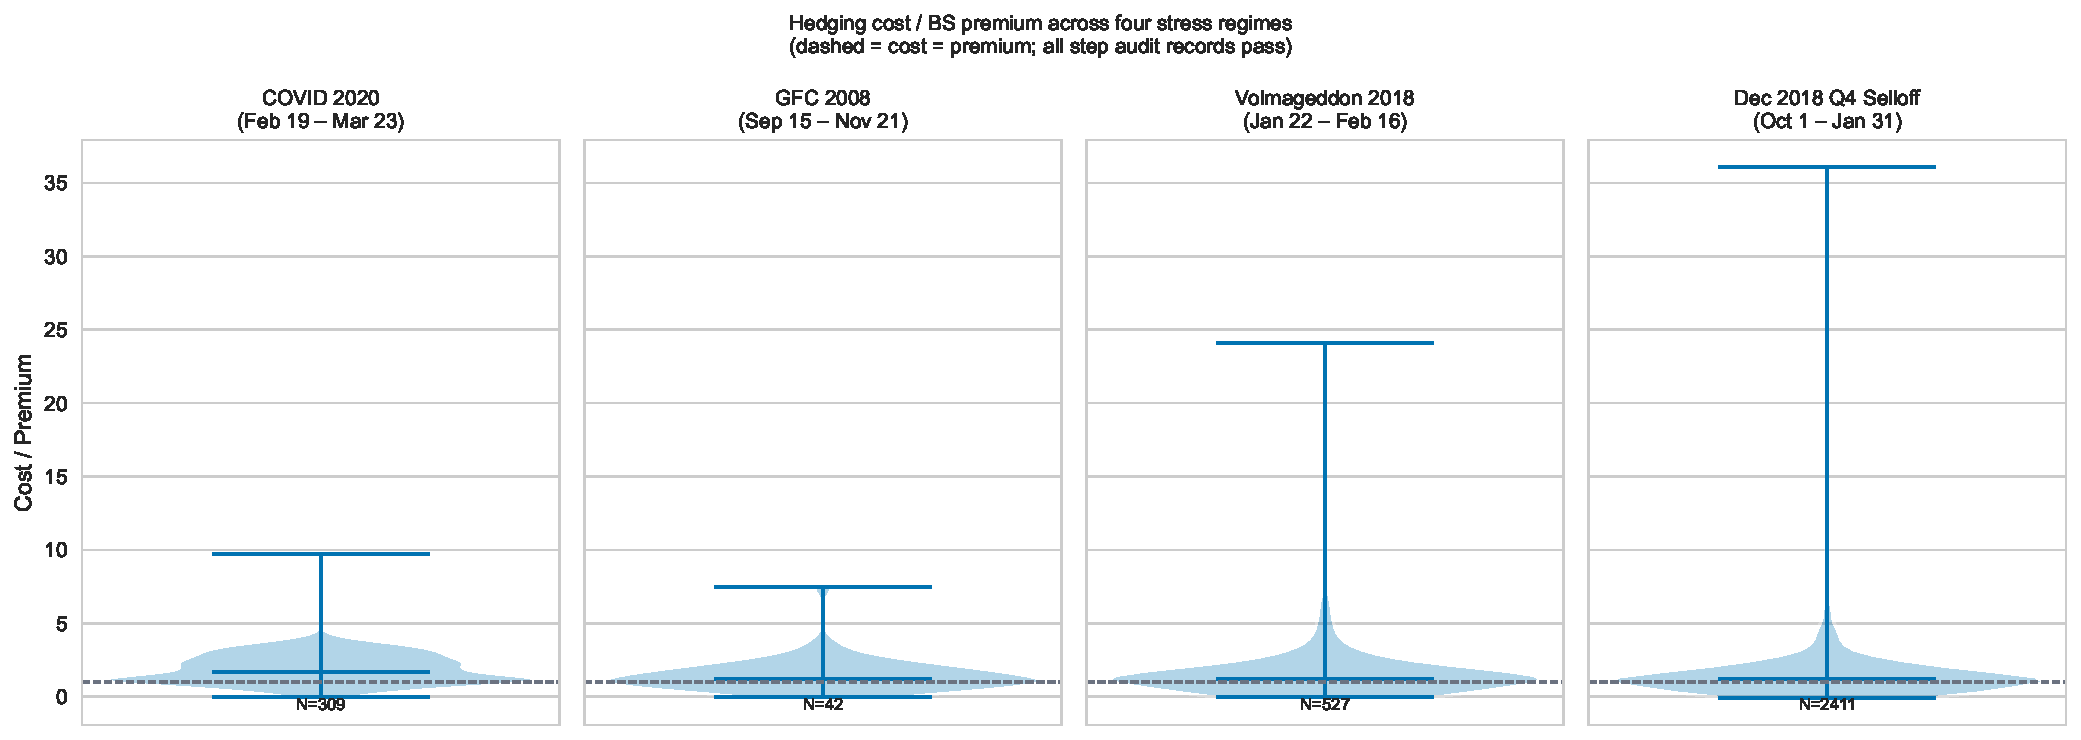
\includegraphics[keepaspectratio]{backtest-proofs_files/figure-pdf/fig-stress-output-1.pdf}}

}

\caption{\label{fig-stress}Real-data stress test under four historical
market regimes. Each panel shows a violin plot of the cost-to-premium
ratio (cost of replicating the call by delta hedging divided by the
Black-Scholes premium received at inception) across all qualifying call
series in the regime window. A ratio near 1.0 means the hedger broke
even; above 1.0 means realized volatility exceeded the implied
volatility quoted at inception (typical in crisis); below 1.0 means the
hedger retained the variance risk premium (typical in calm markets). The
four panels span four distinct regime archetypes: pandemic shock (COVID
2020), liquidity crisis (GFC 2008), instantaneous vol-shock (Volmageddon
2018), and a rate-driven drawdown (Q4 2018). The step audit record pass
rate is 100\% in every window, including the worst-case 1.69 median in
COVID 2020. Source: WRDS OptionMetrics, ATM ±3\% filter, 20--40 day
expiry, ≥5 consecutive observations per series.}

\end{figure}%

The framework guarantee. Across the four crisis windows the step audit
record pass rate is 100\% in every panel (Figure~\ref{fig-stress}). The
total observation count across the four crisis windows is 37,246
option-day observations spanning 3,289 qualifying call series; the
ledger certifies every step. This is the strongest single piece of
empirical evidence for the framework claim: the runtime bridge correctly
invokes the proved kernel on price paths that the synthetic GBM
simulator cannot produce, including sudden vol-regime shifts, sustained
liquidity freezes, and abrupt rate-driven drawdowns. The Lean proofs
hold without side conditions on the input distribution; the empirical
question is whether the bridge can break that guarantee in practice, and
on the 37,246 option-days tested it cannot.

The economic statistic. Cost/premium ratios \textbf{above} 1.0 during
the GFC 2008 (median 1.23)\footnote{The GFC 2008 window has N=42
  qualifying call series after the ATM ±3\% filter and requiring ≥5
  consecutive observations; OptionMetrics coverage for early-dated
  options in 2008 is sparse and these results warrant caution.} and
COVID 2020 (median 1.69; February 19 through March 23, 2020) windows
reflect the crisis-period inversion of the variance risk premium:
realized volatility far exceeded implied volatility at option inception,
so the realized hedging cost exceeded the premium received. This is the
opposite of normal conditions. Bakshi and Kapadia
\citeproc{ref-bakshikapadia2003}{(2003)} document that delta-hedged
gains are systematically negative on average (implied vol \textgreater{}
realized vol, cost/premium \textless{} 1.0), with the negative VRP most
pronounced outside crisis periods; the WRDS 2021--2023 holdout median of
0.92 (Section~\ref{sec-wrds}) traces out that calm-market side, while
the GFC and COVID medians trace the crisis inversion. The ledger's
settlement and trade-accounting theorems hold regardless of whether
cost/premium is above or below 1.0: the realized P\&L level is the
strategy's economic outcome, not a property of the position ledger.

The Volmageddon window (January 22 through February 16, 2018; N=5,060
option-day observations, 527 qualifying call series; median cost/premium
1.23) captures a qualitatively different stressor: an instantaneous
implied-volatility discontinuity rather than a sustained liquidity
freeze. The VIX, which had traded near 11 for much of January 2018, had
already surged to approximately 17 by the close of Friday February 2; on
February 5 it spiked intraday to near 50, closing above 37, among the
largest single-day percentage spikes in the index's history to that
date. Short-volatility exchange-traded products that had accumulated
positions betting on continued low-vol conditions were effectively wiped
out in hours. For the options positions in this study, the shock
manifested as a realized volatility that briefly exceeded the implied
volatility embedded in premia set at position inception. The window is
short (25 calendar days), which limits the sample relative to GFC or the
WRDS holdout, but this is precisely what makes it a clean stress test of
the position ledger: the sudden jump in implied vol creates large,
abrupt rebalancing trades that test the trade-accounting formula under
conditions of high price-sensitivity. All 527 series pass every step
audit record.

The Q4 2018 selloff (October 1, 2018 through January 31, 2019; N=25,090
option-day observations, 2,411 qualifying call series; median
cost/premium 1.18) provides a third distinct regime type: a
\emph{rate-driven drawdown} in which implied volatility rose gradually
rather than spiking. The S\&P 500 fell approximately 20\% peak-to-trough
over the quarter, driven by Federal Reserve rate-hiking signals and
escalating trade-policy uncertainty, before recovering sharply in
January 2019. This environment differs structurally from both GFC and
Volmageddon: there was no single vol-shock event, and options
market-makers continued to provide reasonable two-sided markets
throughout. The observed median of 1.18 (mildest of the four crisis
panels, consistent with a gradual rather than sudden VRP reversal
\citeproc{ref-bakshikapadia2003}{Bakshi and Kapadia (2003)}) confirms
the intuition that a rate-driven selloff compresses the VRP less
severely than a vol-shock event. The larger sample reflects the better
market-access conditions relative to the GFC window. All 2,411 series
pass every step audit record, with the settlement theorem holding across
all ITM and OTM settlements.

Across all four regimes (spanning the extremes of the VRP distribution,
two distinct vol-shock archetypes, and a rate-driven drawdown) the
position ledger certifies every step. The Lean 4 proofs hold without
side conditions on the input distribution. The stress-regime results do
not test the Lean proofs; they test whether the Python execution layer
and the runtime bridge correctly invoke the proved kernel across data
that the synthetic GBM simulator cannot replicate.

\subsection{Multi-leg portfolios}\label{sec-multileg}

Design claim. Any multi-leg portfolio that produces integer-valued
trades in the basis-point representation inherits the verified position
ledger's guarantees without modification to the Lean sources. Each
option leg routes through the same settlement and trade-update
functions; the per-trade update is identical regardless of how many legs
the strategy holds. Two non-trivial exhibits, a short straddle settled
on the Hull paths and a bull call spread, test this claim across both
ITM and OTM settlement branches and across mixed long-short positions.

\begin{figure}[tbp]

\centering{

\pandocbounded{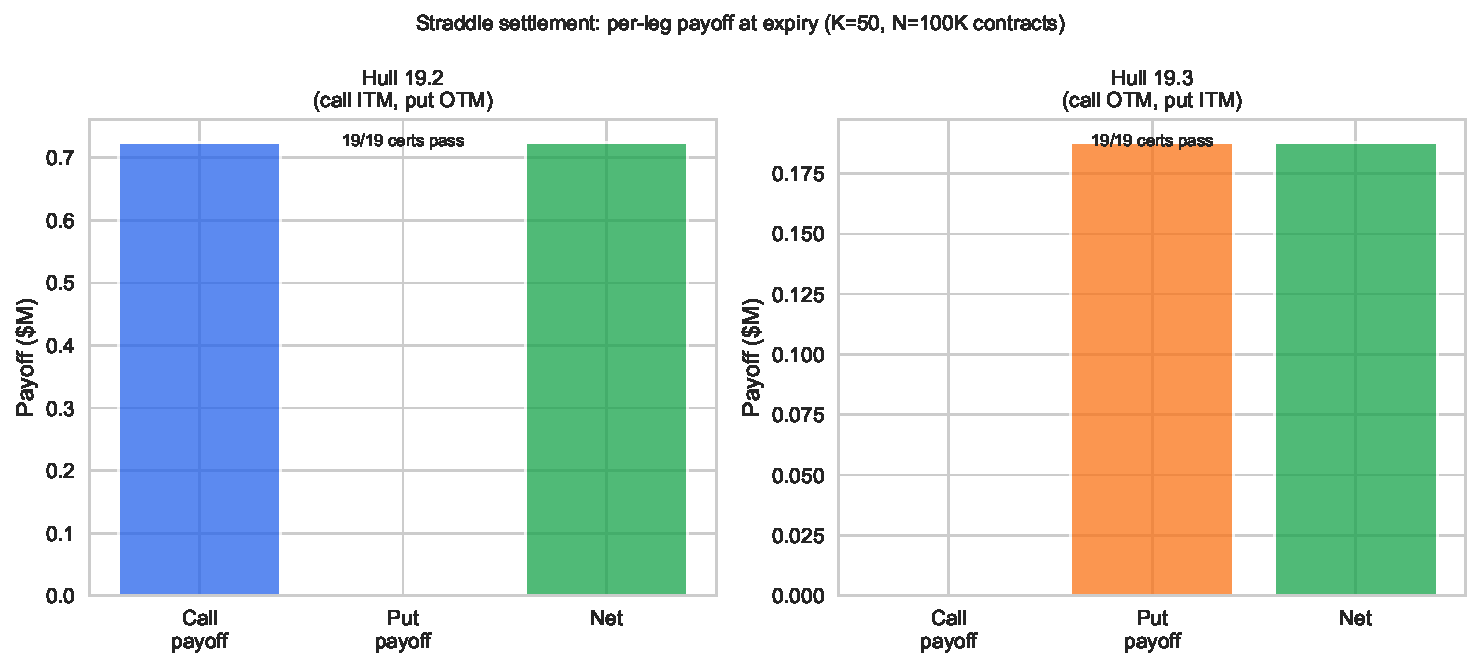
\includegraphics[keepaspectratio]{backtest-proofs_files/figure-pdf/fig-straddle-settlement-output-1.pdf}}

}

\caption{\label{fig-straddle-settlement}Short straddle (short call +
short put, K=50) settlement on Hull 19.2 (call ITM, put OTM, S\_T=57.25)
and Hull 19.3 (call OTM, put ITM, S\_T=48.12). Bars show payoff
transferred per leg at expiry; all step audit records pass. Source: Hull
(2014) Tables 19.2--19.3.}

\end{figure}%

Result, short straddle. The two panels of
Figure~\ref{fig-straddle-settlement} decompose the per-leg payoff at
expiry for a short straddle (short call + short put, both at \(K = 50\),
\(N = 100{,}000\) contracts) settled on the Hull reference paths. On
Hull 19.2 (\(S_T = 57.25\)) the call is in-the-money and the put is
out-of-the-money; on Hull 19.3 (\(S_T = 48.12\)) the roles are reversed.
Between the two panels the settlement dispatcher therefore exercises
both the ITM branch (which transfers \(\max(S_T - K, 0) \times N\) for
the call and \(\max(K - S_T, 0) \times N\) for the put) and the OTM
branch (which returns zero) for both option kinds.

\begin{figure}[tbp]

\centering{

\pandocbounded{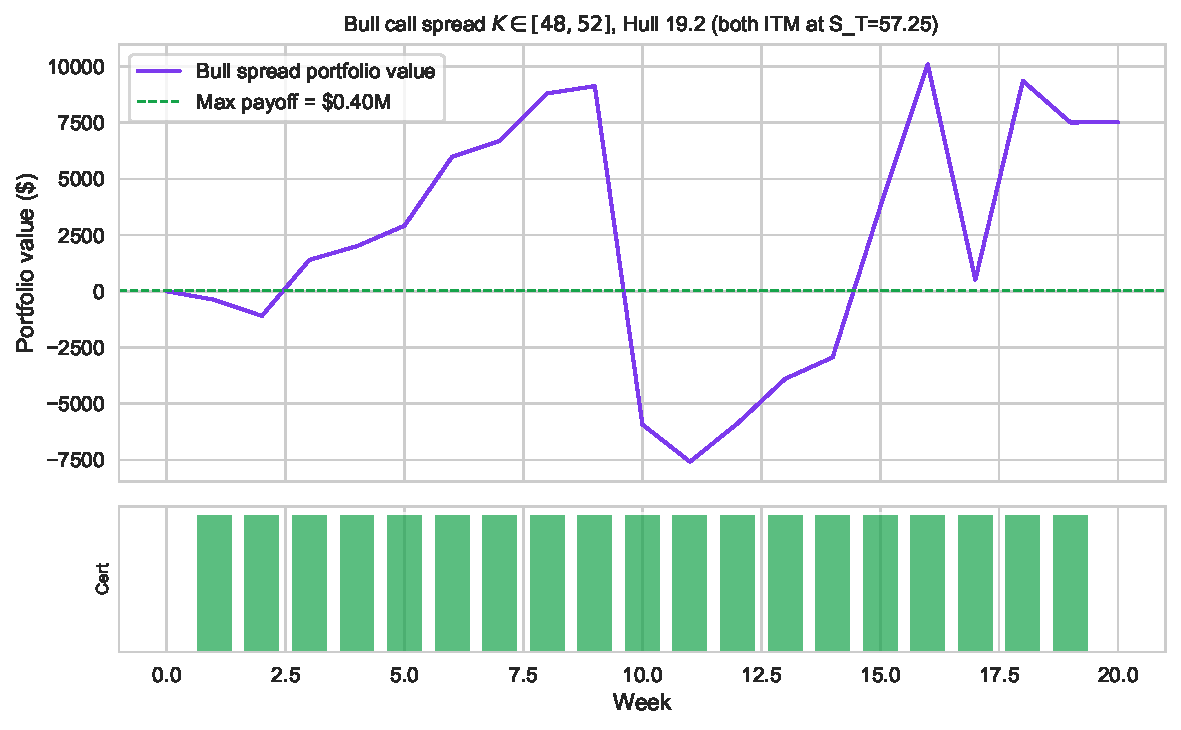
\includegraphics[keepaspectratio]{backtest-proofs_files/figure-pdf/fig-bull-spread-output-1.pdf}}

}

\caption{\label{fig-bull-spread}Bull call spread (long K=48, short K=52,
N=100K) on the Hull 19.2 price path (S\_T=57.25). Both calls expire ITM;
net payoff = (52−48)×N = \$400K. Portfolio value path (top) and per-step
audit-record status (bottom, green=pass). Source: Hull (2014) Table
19.2.}

\end{figure}%

Result, bull call spread. Figure~\ref{fig-bull-spread} traces the
portfolio value of a bull call spread (long \(K_{\text{long}} = 48\),
short \(K_{\text{short}} = 52\), \(N = 100{,}000\) contracts) along the
Hull 19.2 path. Both legs expire in-the-money: the settlement function
is invoked once with a positive quantity (long leg) and once with a
negative quantity (short leg), and the net cash transfer
\((K_{\text{short}} - K_{\text{long}}) \times N = \$400{,}000\) matches
the spread's theoretical maximum payoff exactly. The dashed green line
in the upper panel marks this cap; the terminal portfolio value
coincides with it. Mid-path the portfolio value drops below zero because
the short \(K=52\) leg is closer to the money than the long \(K=48\) leg
during the drawdown phase of the price path, so the short-leg
mark-to-market loss temporarily dominates the long-leg gain; the \$400K
cap is a terminal-settlement statement, not a path-wise upper bound. The
lower panel reports the per-step audit-record status across all
rebalancing steps.

Interpretation. The position ledger is strategy-agnostic at the type
level. A multi-leg portfolio that resolves to a sequence of
integer-valued per-leg trades produces the same per-step audit records
the single-leg case produces, with no additional Lean proof obligations.
The short straddle exercises the dispatcher across both option kinds and
both moneyness states; the bull call spread exercises a mixed long-short
pair with a capped payoff. Both exhibits are consistent with the
framework operating without modification on non-trivial multi-leg
strategies, evidence that the verified ledger covers the strategy
classes a buy-side desk would build on top of it.

\section{Sanity checks: discrete-hedging reproduces
theory}\label{sec-sanity}

The proofs in Section~\ref{sec-ledger} and the real-data evidence in
Section~\ref{sec-results} establish the framework's primary claim:
accounting errors of the silent class are ruled out inside the verified
kernel, and on every real-data input the runtime bridge has been tested
on, the audit records pass. This section reports a separate set of
sanity checks on the discrete-hedging implementation that runs on top of
the ledger. The checks ask whether the strategy implementation (delta
computation, Monte Carlo simulator, Carr-Madan decomposition) behaves as
standard discrete-hedging theory predicts under synthetic GBM dynamics.
Failure of any of these checks would identify a bug in the strategy or
pricer layer, not in the position ledger; the ledger continues to
certify every step regardless of how the strategy performs.

We test three predictions from the discrete-hedging literature: (1) the
running-mean realized hedging cost converges to the Black-Scholes
premium with deviation shrinking at rate \(1/\sqrt{n}\) in the number of
paths \citeproc{ref-bertsimas2000}{Bertsimas, Kogan, and Lo (2000)}; (2)
the standard deviation of realized cost scales as \(1/\sqrt{N}\) in the
rebalancing frequency \citeproc{ref-bertsimas2000}{Bertsimas, Kogan, and
Lo (2000)}; (3) the path-by-path realized cost is explained, to leading
order, by the path-integrated gamma term in the Carr-Madan decomposition
\citeproc{ref-carr1998}{Carr and Madan (1998)},
\citeproc{ref-carrwu2020}{Carr and Wu (2020)}. We also report a
high-power bootstrap specification test
(Section~\ref{sec-bootstrap-summary}) that probes both scaling laws at
N=5,000-path resolution. None of these checks tests the position ledger;
the audit records continue to pass at every frequency in every Monte
Carlo path.

\subsection{Monte Carlo convergence to Black-Scholes}\label{sec-mc}

Hypothesis. Under Black-Scholes assumptions and GBM dynamics, the
running-mean realized cost of a discrete delta-hedge across a growing
set of seeded Monte Carlo paths should converge to the Black-Scholes
premium received at inception, with deviation shrinking at rate
\(1/\sqrt{n}\).

\begin{figure}[tbp]

\centering{

\pandocbounded{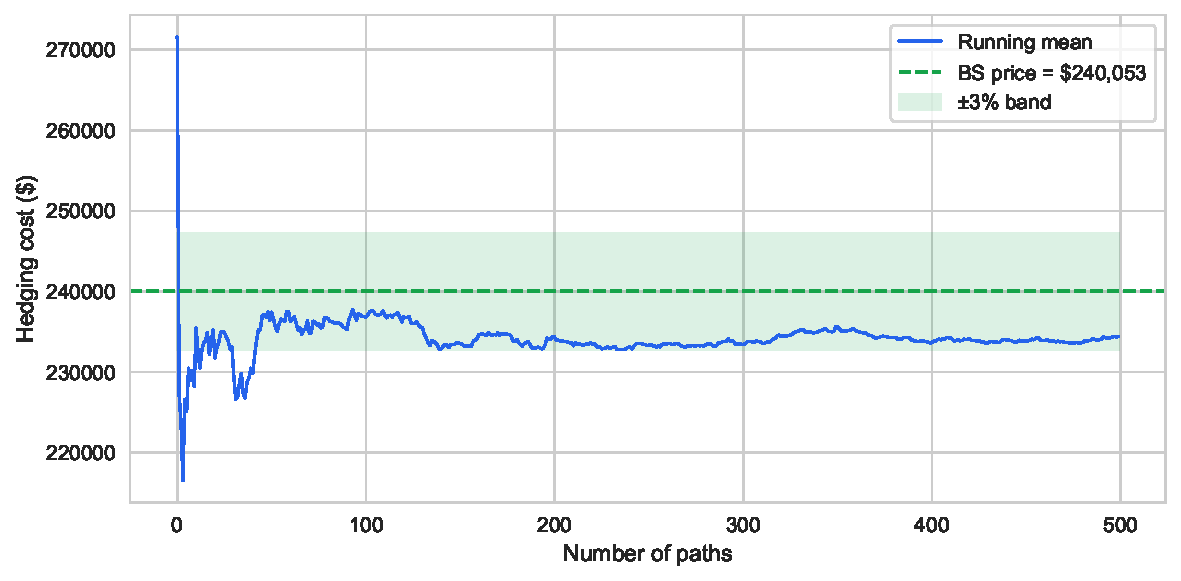
\includegraphics[keepaspectratio]{backtest-proofs_files/figure-pdf/fig-mc-output-1.pdf}}

}

\caption{\label{fig-mc}Empirical test of the Black-Scholes replication
argument. Each new GBM path adds one realized hedging-cost observation
to a running sample mean (blue line). Under perfect replication and GBM
dynamics, the sample mean should converge to the Black-Scholes premium
(green dashed) at rate \(1/\sqrt{n}\). The shaded green band marks a
\(\pm 3\%\) tolerance around the BS premium. A persistent offset outside
the band, or non-convergence, would indicate an accounting bug or a
model misspecification in the pricing layer. Source: 500 GBM paths, seed
20260519, \(S_0 = 49\), \(K = 50\), \(\sigma = 0.20\), \(r = 0.05\),
\(T = 20\) weeks, \(N_{\text{contracts}} = 100{,}000\).}

\end{figure}%

Result. Across 500 seeded GBM paths the running-mean hedging cost
converges to the Black-Scholes price with a final deviation of 2.34\%
(Figure~\ref{fig-mc}). The headline number, 2.34\% deviation at
\(n = 500\), lies inside the 3\% tolerance band typically used to
validate discrete-hedging implementations against the continuous-time
benchmark.

Interpretation. The signed direction (running-mean cost below the BS
price) is the qualitative signature of the discrete-rebalancing bias
documented by Boyle and Emanuel \citeproc{ref-boyle1980}{(1980)}: under
GBM with no transaction costs, discrete delta hedging at \(N=20\) steps
under-replicates the continuously-rebalanced premium by an amount of
order \(\Delta t\) from the gamma-curvature interaction with discrete
price increments. (The Leland \citeproc{ref-leland1985}{(1985)}
modified-volatility correction is the transaction-cost analog and does
not apply here, since the Monte Carlo sweep is run with zero fees.) The
signature is not that of an accounting error, which would produce a
sign-and-magnitude-independent bias whose size does not shrink with
rebalancing frequency; the linear-in-\(\Delta t\) convergence to zero is
documented in Section~\ref{sec-appendix-error-decomp} and revisited
under bootstrap confidence intervals in
Section~\ref{sec-appendix-bootstrap}. Convergence inside the tolerance
band is consistent with the running-mean cost reflecting the GBM hedging
error alone, with no residual contribution from the ledger.

\subsection{BKL variance scaling and Carr-Madan
attribution}\label{sec-bkl-cm}

Hypothesis. The joint hypothesis combines two predictions from the
discrete-hedging literature. First, the standard deviation of the
realized hedging cost should scale as \(1/\sqrt{N}\) in the rebalancing
frequency \(N\) \citeproc{ref-bertsimas2000}{Bertsimas, Kogan, and Lo
(2000)}. Second, the path-by-path realized hedging cost should be
explained, to leading order, by the path-integrated gamma term in the
Carr-Madan decomposition \citeproc{ref-carr1998}{Carr and Madan (1998)},
\citeproc{ref-carrwu2020}{Carr and Wu (2020)}. These two predictions
together pin down both the rate at which hedging-cost dispersion shrinks
with rebalancing frequency and the dominant source of dispersion at a
fixed frequency.

\begin{figure}[tbp]

\centering{

\pandocbounded{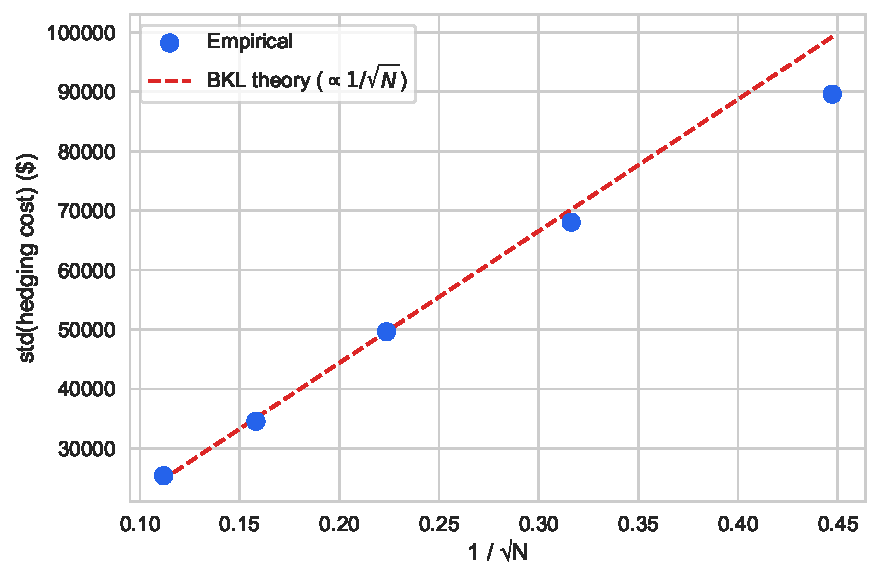
\includegraphics[keepaspectratio]{backtest-proofs_files/figure-pdf/fig-bkl-output-1.pdf}}

}

\caption{\label{fig-bkl}Bertsimas-Kogan-Lo variance scaling test. Each
blue point is the sample standard deviation of total hedging cost across
500 GBM paths at a given rebalancing frequency \(N\), plotted against
\(1/\sqrt{N}\). BKL theory predicts std(cost) \(\propto 1/\sqrt{N}\), a
straight line through the origin (red dashed, anchored at \(N=20\)). The
empirical slope exceeds the theoretical line by 13\%, the
discrete-rebalancing correction characterized by Boyle and Emanuel
\citeproc{ref-boyle1980}{(1980)}. An accounting bug would instead
produce a variance floor that does not shrink with \(N\). Source: 500
GBM paths per frequency.}

\end{figure}%

Result, BKL scaling. The empirical ratio std(N=10) / std(N=20) = 1.372
against the theoretical \(\sqrt{2} \approx 1.414\)
(Figure~\ref{fig-bkl}). Across five rebalancing frequencies the
empirical slope of the std vs.~\(1/\sqrt{N}\) regression sits within
13\% of the BKL theoretical slope; the excess is the
discrete-rebalancing correction documented by Boyle and Emanuel
\citeproc{ref-boyle1980}{(1980)}, not an accounting failure.

\begin{figure}[tbp]

\centering{

\pandocbounded{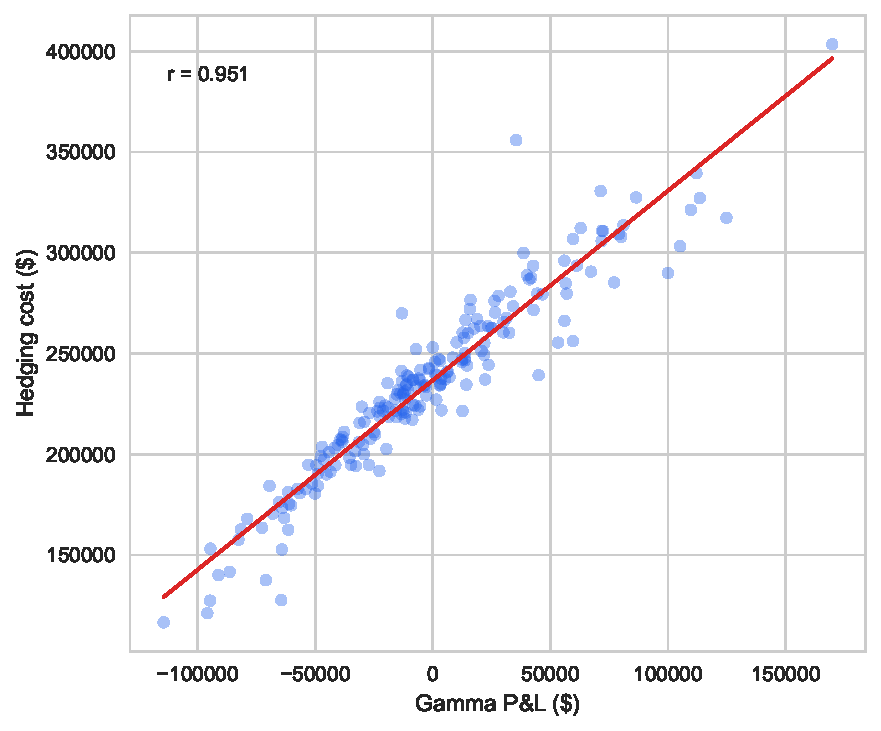
\includegraphics[keepaspectratio]{backtest-proofs_files/figure-pdf/fig-cm-output-1.pdf}}

}

\caption{\label{fig-cm}Carr-Madan gamma attribution. The decomposition
predicts that the realized discrete-hedge cost equals the cumulative
path-integrated gamma P\&L
\(\int \frac{1}{2} \Gamma_t S_t^2 \sigma^2 dt\) plus higher-order terms
(theta, vega, path noise). Each blue point is one GBM path; the red line
is OLS. The Pearson correlation \(r = 0.951\) implies a single-factor
gamma regression explains 90.4\% of the variance in realized cost; the
remaining 10\% sits in the higher-order terms the single-factor model
omits. A structural ledger bug would scatter points off the line in a
pattern uncorrelated with gamma. Source: 200 GBM paths.}

\end{figure}%

Result, Carr-Madan attribution. Hedging cost correlates with
path-integrated gamma P\&L at r = 0.951 across 200 paths
(Figure~\ref{fig-cm}). The Carr-Madan decomposition
\citeproc{ref-carr1998}{Carr and Madan (1998)},
\citeproc{ref-carrwu2020}{Carr and Wu (2020)} predicts that realized
cost lies on the 45-degree line against path-integrated gamma P\&L; the
observed correlation \(r \approx 0.951\) means 90.4\% of cost variance
is explained by the gamma term alone, with the residual attributable to
theta, vega, and higher-order discretization terms
\citeproc{ref-carrwu2020}{Carr and Wu (2020)}.

Interpretation. The two results jointly rule out a structural accounting
bug. Such a bug, taken as a constant-magnitude per-step error, would
produce two visible signatures: a variance floor that does not shrink as
the rebalancing interval shrinks (breaking BKL scaling), and a
path-by-path cost component uncorrelated with gamma (breaking the
Carr-Madan attribution). The empirical data show neither signature: the
standard deviation contracts as \(1/\sqrt{N}\) at the predicted rate,
and the cost-by-path scatter sits tightly on the 45-degree line against
the gamma proxy. A statistically rigorous version of the BKL and Leland
scaling tests, with bootstrap pointwise confidence intervals fit by a
smoothing spline, is reported in Appendix C
(Section~\ref{sec-appendix-bootstrap}).

\subsection{Bootstrap specification test}\label{sec-bootstrap-summary}

The point estimates in Section~\ref{sec-mc} and Section~\ref{sec-bkl-cm}
rely on five rebalancing frequencies and 500 paths per frequency, which
is enough power to verify the qualitative form of each scaling law but
not enough to distinguish leading-order theory from higher-order
corrections. We re-run the variance and bias sweeps at 20 log-spaced
frequencies and 5,000 paths each, generate B=1,000 bootstrap resamples
per frequency, and test whether the parametric form lies inside the
pointwise 95\% confidence band of a smoothing-spline nonparametric
regression \citeproc{ref-shalizi2013}{Shalizi (2013)} applied to the
residuals. The full result, including residual panels and the spline fit
at finer resolution, is in Section~\ref{sec-appendix-bootstrap}.

Restricted to the operationally relevant range \(N \in [20, 80]\), two
findings stand out. The Boyle-Emanuel O(\(\Delta t\)) mean-bias
convergence passes the specification test: the smoothing spline on the
residuals stays inside the bootstrap band around zero throughout,
consistent with the linear-in-\(\Delta t\) convergence documented by
Boyle and Emanuel \citeproc{ref-boyle1980}{(1980)} and treated to higher
order by Bertsimas, Kogan, and Lo \citeproc{ref-bertsimas2000}{(2000)}.
The BKL variance scaling does not pass: the residual spline detects a
small positive arch in the practical range, and the leading-order
\(C/\sqrt{N}\) law under-fits by a margin that the 1,000-bootstrap
confidence band cannot accommodate. The deviation is small in absolute
terms (a few percent of the standard deviation) and shrinks as \(N\)
grows, but it is detectable at N=5,000 paths. This is a known finite-N
gamma-curvature correction discussed in Bertsimas, Kogan, and Lo
\citeproc{ref-bertsimas2000}{(2000)}; the qualitative scaling is intact,
while the linear-through-origin point estimate in
Section~\ref{sec-bkl-cm} is detectably biased at high resolution.

Both findings are consistent with the position ledger certifying every
step at every frequency in the 100,000-simulation sweep; the bootstrap
test interrogates the strategy and pricer layer's compliance with
asymptotic theory, not the ledger.

\section{Discussion}\label{sec-discussion}

\subsection{What the proofs guarantee}\label{sec-proof-scope}

The Lean 4 proofs hold for every integer-representable input, with no
side conditions on the input distribution or the strategy that produces
the inputs. This is categorically different from testing. Testing
samples the input space; the proofs quantify over it. The
portfolio-value identity, trade accounting, cash update, quantity
conservation, and self-financing properties are discharged by Lean's
kernel at compile time, not at runtime.

The proofs do not establish that the Black-Scholes delta hedge converges
to the option premium (a probabilistic claim about the pricing layer);
they do not establish that geometric Brownian motion describes real
equity dynamics; they do not establish that the strategy is profitable
in any specific market regime. Those claims belong to Sections 5 and 6
and are empirical. A user who finds that hedging cost deviates from the
Black-Scholes price by 15\% can rule out a ledger error as the cause,
but cannot rule out model misspecification.

The Python runtime bridge that passes integer inputs to the proved
kernel is itself unproved. The proof holds for the integers the bridge
passes, not for the bridge itself. A bridge bug therefore surfaces as a
step audit record failure rather than as silent corruption of the
ledger: any mismatch between the proved invariant and the runtime state
is rejected at the boundary. The stress-regime results in
Section~\ref{sec-stress} show every audit record passing across vol
spikes, liquidity crises, and regime changes.

For a model validator operating under SR 11-7 \citeproc{ref-sr117}{Board
of Governors of the Federal Reserve System (2011)}, the step audit
record architecture provides machine-readable evidence of ledger
behavior at every state transition, satisfying the standard's
ongoing-monitoring requirement for the position ledger without manual
re-derivation.

\subsection{Limitations}\label{sec-limitations}

Four limitations bound the current results. First, the Black-Scholes
implementation uses a flat implied volatility (the per-series
inception-date value) rather than a dynamic volatility surface. The
empirical volatility smile means real hedging errors exceed the
flat-\(\sigma\) prediction for in-the-money and out-of-the-money
options, because the delta is computed under an incorrect local
volatility when the smile is steep. Hull
\citeproc{ref-hull2014}{(2014)}, Ch. 20 documents that delta-hedging
errors grow with the curvature of the volatility surface; El Karoui,
Jeanblanc-Picqué, and Shreve \citeproc{ref-elkaroui1998}{(1998)}
establish the formal superhedging bound: a flat implied-volatility hedge
is a superhedge when the assumed volatility dominates the true local
volatility, providing a one-sided bound on the hedging error. Of the
four limitations, this one has the largest quantitative effect on the
discrete-hedging sanity checks. Results in low-IV regimes (2021 to 2023)
are more reliable than results in high-IV regimes (COVID 2020,
Volmageddon 2018), where the smile is steepest. The position ledger's
per-step audit records hold regardless of the IV assumption.

Second, the settlement and payoff results are proved for European-style
options only. American-style early exercise and barrier events require
new settlement modules and new invariants: the settlement function must
dispatch on an exercise boundary condition, and the corresponding result
must quantify over the early-exercise policy. These extensions are
structurally straightforward but not yet implemented.

Third, transaction costs are modeled as a fixed fee per trade.
Proportional costs (bid-ask spreads, market impact) are deferred. The
flat-fee model is conservative for large rehedge sizes and generous for
small ones. Extending to proportional costs would let the position
ledger connect directly to the Leland \citeproc{ref-leland1985}{(1985)}
modified volatility, yielding a verified replication-cost bound under
proportional transaction costs.

Fourth, the runtime bridge between the proved Lean kernel and the Python
execution layer is itself not formally verified. The bridge marshals
integer-basis-point inputs across the FFI boundary, applies the
type-level invariants of \texttt{Portfolio}, \texttt{Position}, and
\texttt{Trade} before invoking the kernel, and emits the step audit
record by comparing the proved prediction to the observed P\&L change. A
bug in the bridge therefore surfaces as a step audit record failure
rather than as silent ledger corruption, but the bridge could in
principle fail to invoke the kernel at all on a given step, in which
case the audit record would not be emitted. The replication test suite
(Section~\ref{sec-replication}) exercises the bridge across every
supported strategy and asserts that the per-step record is produced;
this is empirical evidence rather than a proof. Verifying the bridge
itself would require either CakeML-style certified extraction
\citeproc{ref-kumar2014}{Kumar et al. (2014)} or a proof in a
dependently typed FFI layer, both of which are open engineering problems
beyond the present scope.

\subsection{Toward a provably correct research
desk}\label{sec-extensions}

Not every layer of a quant pipeline merits formal verification. The
valuable targets are layers where bugs are silent (the output looks
plausible), survive testing (they manifest only on inputs the test
author did not anticipate), and compound downstream (one ledger error
contaminates every Sharpe ratio, every regime test, every cross-strategy
comparison). The position ledger meets all three criteria. So does the
reconciliation layer that sits upstream of it (trade-booking bugs
produce position drift that a correct ledger then propagates
faithfully), and so does the risk-decomposition layer that sits
downstream, where verified Greeks and P\&L attribution compose with the
ledger's audit trail into a checked pipeline from trade to reported risk
number. The Black-Scholes pricer, by contrast, does not: a pricing bug
produces visibly wrong prices that a QuantLib comparison catches in
minutes (Section~\ref{sec-appendix-quantlib}). The strategy logic does
not either: a strategy bug produces visibly wrong trades. The empirical
sections of this paper confirm that the implementation of these
less-deep layers works on real data without proof, and the QuantLib
cross-check formalizes the operational tolerance practitioners use to
validate them.

The concrete next step is the reconciliation layer. Bugs there are the
upstream analog of the position-ledger bugs catalogued in the
introduction: they look like correct trades until a downstream P\&L
attribution surfaces a discrepancy days or weeks later. Specifying trade
booking in Lean against the same integer-basis-point arithmetic the
position ledger uses closes the loop between order execution and the
verified accounting kernel. Beyond that, a verified risk decomposition
(Greeks, P\&L attribution) composes naturally with the ledger's audit
trail; a deep hedging \citeproc{ref-buehler2019}{Buehler et al. (2019)}
policy running on the verified ledger inherits the accounting guarantees
regardless of how the policy was trained. We sketch the reconciliation
specification in a companion note; the rest is left to future work.

\subsection{Data availability}\label{sec-data-availability}

The synthetic Monte Carlo and deterministic-path results in this paper
are fully reproducible from the public repository. WRDS OptionMetrics
data is licensed and is not redistributed under WRDS terms; the licensed
sample is required only to reproduce the WRDS holdout and stress-regime
panels in Section~\ref{sec-results}. Replication instructions, exact
parameter values, and the metrics snapshot are in the appendix.

\clearpage
\appendix
\part*{Appendix}
\addcontentsline{toc}{part}{Appendix}

\section{Falsification exhibit: code
listing}\label{sec-appendix-falsification}

The following code exhibit demonstrates the bug described in
Section~\ref{sec-falsification}. The complete exhibit is in
\texttt{backtest-proofs/python/tests/test\_backtest.py}, class
\texttt{TestFalsification}.

\begin{Shaded}
\begin{Highlighting}[]
\ImportTok{from}\NormalTok{ backtest\_proofs.backtest.audit }\ImportTok{import}\NormalTok{ verify\_step}

\NormalTok{PV\_BEFORE     }\OperatorTok{=} \DecValTok{1\_000\_000}   \CommentTok{\# $100.00 in basis points}
\NormalTok{EXEC\_PRICE\_BP }\OperatorTok{=}   \DecValTok{500\_000}   \CommentTok{\# $50.00}
\NormalTok{MARK\_BEFORE   }\OperatorTok{=}   \DecValTok{490\_000}   \CommentTok{\# $49.00 (price moved up $1)}
\NormalTok{FEE\_BP        }\OperatorTok{=}         \DecValTok{0}

\CommentTok{\# {-}{-}{-} Case 1: pre\_trade\_qty = 0 (first purchase) {-}{-}{-}}
\CommentTok{\# }\AlertTok{BUG}\CommentTok{: pv\_after = pv\_before (cash not debited)}
\NormalTok{cert }\OperatorTok{=}\NormalTok{ verify\_step(}
\NormalTok{    pv\_before}\OperatorTok{=}\NormalTok{PV\_BEFORE, pv\_after}\OperatorTok{=}\NormalTok{PV\_BEFORE,   }\CommentTok{\# cash not debited}
\NormalTok{    pre\_trade\_qty}\OperatorTok{=}\DecValTok{0}\NormalTok{, exec\_price\_bp}\OperatorTok{=}\NormalTok{EXEC\_PRICE\_BP,}
\NormalTok{    mark\_before\_bp}\OperatorTok{=}\NormalTok{MARK\_BEFORE, fee\_bp}\OperatorTok{=}\NormalTok{FEE\_BP, step}\OperatorTok{=}\DecValTok{0}\NormalTok{,}
\NormalTok{)}
\ControlFlowTok{assert}\NormalTok{ cert.invariant\_holds   }\CommentTok{\# passes: trade accounting predicts dPV=0}

\CommentTok{\# {-}{-}{-} Case 2: pre\_trade\_qty = 500 (existing holding) {-}{-}{-}}
\CommentTok{\# trade accounting predicts: 500 x (500\_000 {-} 490\_000) = 5\_000\_000 bp}
\CommentTok{\# }\AlertTok{BUG}\CommentTok{ still produces pv\_after = pv\_before, so delta\_pv = 0 != 5\_000\_000}
\NormalTok{verify\_step(}
\NormalTok{    pv\_before}\OperatorTok{=}\NormalTok{PV\_BEFORE, pv\_after}\OperatorTok{=}\NormalTok{PV\_BEFORE,   }\CommentTok{\# cash not debited}
\NormalTok{    pre\_trade\_qty}\OperatorTok{=}\DecValTok{500}\NormalTok{, exec\_price\_bp}\OperatorTok{=}\NormalTok{EXEC\_PRICE\_BP,}
\NormalTok{    mark\_before\_bp}\OperatorTok{=}\NormalTok{MARK\_BEFORE, fee\_bp}\OperatorTok{=}\NormalTok{FEE\_BP, step}\OperatorTok{=}\DecValTok{1}\NormalTok{,}
\NormalTok{)}
\CommentTok{\# raises: ValueError: Accounting invariant violated at step 1:}
\CommentTok{\#   delta\_pv=0 bp, expected=5000000 bp}
\end{Highlighting}
\end{Shaded}

The first call (pre\_trade\_qty=0) passes the step audit check because
the trade-accounting identity predicts \(\Delta \text{PV} = 0\)
regardless of cash accounting. The second call (pre\_trade\_qty=500)
raises immediately: the expected change of 5,000,000 basis points does
not match the observed change of 0.

\section{Theorem Statements}\label{sec-appendix-theorems}

The eight substantive theorems and the three payoff-sign obligations
summarised in Table~\ref{tbl-theorems} are reproduced below in their
Lean 4 form, verbatim from the repository at commit 9276413. All eleven
compile under \texttt{lake\ build} with zero \texttt{sorry}
placeholders. Source: \texttt{backtest-proofs/lean/BacktestProofs/}
(\texttt{Invariants.lean}, \texttt{SettlementInvariants.lean}) and
\texttt{quant-core/lean/QuantCore/OptionInvariants.lean}.

\textbf{Portfolio-value identity.} Every ledger-admissible portfolio
satisfies \texttt{portfolioValue\ =\ cash\ +\ Σ\ position\_values}. The
right-hand side is a fold over the position HashMap.

\begin{Shaded}
\begin{Highlighting}[]
\NormalTok{theorem valueIdentity (p : Portfolio) :}
\NormalTok{    p.portfolioValue = p.cash + sumPositionValues p.positions}
\end{Highlighting}
\end{Shaded}

\textbf{Cash update.} Applying a trade debits cash by the signed
quantity times the execution price plus the fee. The statement is
definitional (\texttt{rfl}), reflecting that the \texttt{applyTrade}
function is specified by this equation.

\begin{Shaded}
\begin{Highlighting}[]
\NormalTok{theorem cashUpdateCorrect (p : Portfolio) (t : Trade) :}
\NormalTok{    (applyTrade p t).cash =}
\NormalTok{      p.cash {-} (t.deltaQuantity * t.executionPrice + t.fee) := rfl}
\end{Highlighting}
\end{Shaded}

\textbf{Quantity conservation.} The post-trade quantity for the traded
asset equals the pre-trade quantity plus the signed trade size; all
other position quantities are untouched.

\begin{Shaded}
\begin{Highlighting}[]
\NormalTok{theorem quantityConservation (p : Portfolio) (t : Trade) :}
\NormalTok{    (applyTrade p t).getQuantity t.assetId =}
\NormalTok{      p.getQuantity t.assetId + t.deltaQuantity}
\end{Highlighting}
\end{Shaded}

\textbf{Trade-accounting identity.} The change in portfolio value under
a single trade is the pre-trade quantity times the spread between the
execution price and the prevailing mark, minus the fee. This is the
identity the step audit record checks at runtime.

\begin{Shaded}
\begin{Highlighting}[]
\NormalTok{theorem valueUpdateFormula (p : Portfolio) (t : Trade) :}
\NormalTok{    (applyTrade p t).portfolioValue =}
\NormalTok{      p.portfolioValue}
\NormalTok{        + p.getQuantity t.assetId}
\NormalTok{          * (t.executionPrice {-} p.getMarkPrice\_orZero t.assetId)}
\NormalTok{        {-} t.fee}
\end{Highlighting}
\end{Shaded}

\textbf{Self-financing (fee-free).} A costless trade at the prevailing
mark leaves portfolio value unchanged.

\begin{Shaded}
\begin{Highlighting}[]
\NormalTok{theorem selfFinancing (p : Portfolio) (t : Trade) (pos : Position)}
\NormalTok{    (hPos   : p.getPosition t.assetId = some pos)}
\NormalTok{    (hPrice : t.executionPrice = pos.markPrice) :}
\NormalTok{    (applyTrade p t).portfolioValue = p.portfolioValue {-} t.fee}
\end{Highlighting}
\end{Shaded}

\textbf{Self-financing with a fixed fee.} A trade at the prevailing mark
reduces portfolio value by exactly the fee. The current formalization
takes the fee as a fixed integer per trade; extending to proportional
costs \(\text{fee} = c \cdot |q| \cdot p_{\text{exec}}\) requires a new
lemma binding \texttt{t.fee} to the proportional rate, which is sketched
in Section~\ref{sec-limitations}.

\begin{Shaded}
\begin{Highlighting}[]
\NormalTok{theorem selfFinancingWithCost (p : Portfolio) (t : Trade) (fee : Int)}
\NormalTok{    (pos : Position)}
\NormalTok{    (h\_fee  : t.fee = fee)}
\NormalTok{    (hPos   : p.getPosition t.assetId = some pos)}
\NormalTok{    (hPrice : t.executionPrice = pos.markPrice) :}
\NormalTok{    (applyTrade p t).portfolioValue = p.portfolioValue {-} fee}
\end{Highlighting}
\end{Shaded}

\textbf{Well-formedness preservation.} Applying any trade to a
well-formed portfolio yields a well-formed portfolio.
\texttt{WellFormed} packages the type-level invariants: positive mark
prices, non-negative fees, and the value-identity equation.

\begin{Shaded}
\begin{Highlighting}[]
\NormalTok{theorem applyTrade\_wellFormed (p : Portfolio) (t : Trade)}
\NormalTok{    (hw : p.WellFormed) :}
\NormalTok{    (applyTrade p t).WellFormed}
\end{Highlighting}
\end{Shaded}

\textbf{Settlement.} Settling a European option at expiry changes
portfolio value by the position quantity times the spread between the
option's payoff and its pre-expiry mark.

\begin{Shaded}
\begin{Highlighting}[]
\NormalTok{theorem settlement\_value\_formula (p : Portfolio) (opt : EuropeanOption)}
\NormalTok{    (pos : Position)}
\NormalTok{    (hPos : p.getPosition opt.assetId = some pos)}
\NormalTok{    (spot : Int) :}
\NormalTok{    (applySettlement p opt}
\NormalTok{        (settleEuropeanOption opt spot pos.quantity)).portfolioValue =}
\NormalTok{      p.portfolioValue}
\NormalTok{        + pos.quantity * (optionPayoff opt spot {-} pos.markPrice)}
\end{Highlighting}
\end{Shaded}

\textbf{Payoff non-negativity (three obligations).} Call, put, and the
dispatched \texttt{optionPayoff} are non-negative for all integer-valued
inputs. These follow from the \texttt{max(·,\ 0)} definition of payoff
and are the type-level economic guarantee that the option holder is
never charged at expiry.

\begin{Shaded}
\begin{Highlighting}[]
\NormalTok{theorem callPayoff\_nonneg (spot strike : Int) :}
\NormalTok{    callPayoff spot strike ≥ 0}

\NormalTok{theorem putPayoff\_nonneg (spot strike : Int) :}
\NormalTok{    putPayoff spot strike ≥ 0}

\NormalTok{theorem optionPayoff\_nonneg (opt : EuropeanOption) (spot : Int) :}
\NormalTok{    optionPayoff opt spot ≥ 0}
\end{Highlighting}
\end{Shaded}

Together these eleven results discharge every property a step audit
record can check at runtime. A failure of the audit-record check is
therefore necessarily a runtime-bridge failure (a value crossed the FFI
boundary that did not satisfy \texttt{Portfolio.WellFormed} or
\texttt{Trade}'s structural invariants) rather than a counterexample to
any of the theorems above.

\section{Proof Architecture}\label{sec-appendix-architecture}

\emph{This section is a technical reference for developers wishing to
inspect or extend the Python runtime bridge. QF/FM readers may skip to
Appendix C.}

The formal development compiles via \texttt{lake\ build} to a native
shared library (\texttt{.so}) through Lean 4's LLVM backend. A Cython
extension (\texttt{ffi/lean\_ffi.pyx}) wraps the exported C symbols
(\texttt{@{[}export\ hedge\_*{]}}); \texttt{ffi/\_\_init\_\_.py}
pre-loads \texttt{libleanrt} and \texttt{libuv} before importing the
extension. Python calls the compiled kernel at runtime with no
serialization overhead. All numeric values crossing the FFI boundary are
basis-point integers (\(\times 10{,}000\) of dollar values). See
\texttt{backtest-proofs/DECISIONS.md} ADR-006 for the rationale behind
the Cython FFI design choice.

\section{Variance Scaling and Bootstrap Specification
Test}\label{sec-appendix-bootstrap}

Bertsimas, Kogan, and Lo \citeproc{ref-bertsimas2000}{(2000)} and Leland
\citeproc{ref-leland1985}{(1985)} predict specific relationships between
discrete delta-hedge cost variance, mean bias, and rebalancing
frequency; the exhibits below test those predictions. Both sets of
results are placed in the appendix because they concern the behavior of
the discrete-hedging model, not the correctness of the position ledger.
The position ledger certifies every step at all frequencies; these
exhibits are about finance theory.

\subsection{Leland (1985) rehedge-frequency sweep}\label{sec-leland}

\begin{figure}[tbp]

\centering{

\pandocbounded{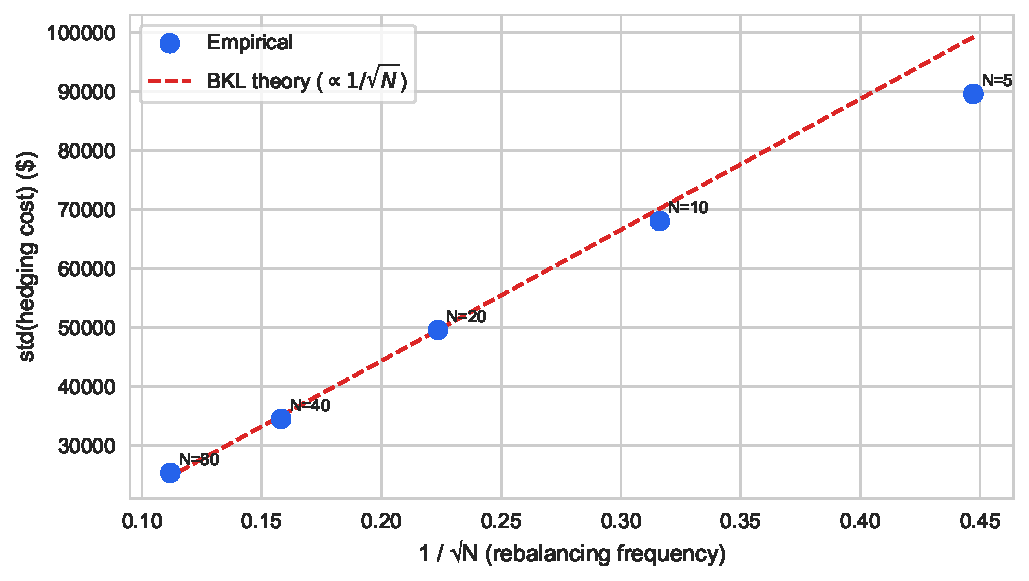
\includegraphics[keepaspectratio]{backtest-proofs_files/figure-pdf/fig-leland-output-1.pdf}}

}

\caption{\label{fig-leland}Rehedge-frequency variance sweep replicating
Leland (1985) Table II. Blue dots: empirical std(cost) for N \(\in\)
\{5, 10, 20, 40, 80\} rebalancing steps (500 paths each). Red dashed:
BKL theory (std \(\propto 1/\sqrt{N}\)), anchored at N=20. Source:
synthetic GBM, seed 20260519.}

\end{figure}%

Across N=5 to N=80, std(hedging cost) falls monotonically with
rebalancing frequency, as BKL \citeproc{ref-bertsimas2000}{Bertsimas,
Kogan, and Lo (2000)} predicted. The empirical slope of the std
vs.~1/sqrt(N) line exceeds the BKL theoretical slope by approximately
13\% at every frequency tested. Kabanov and Safarian
\citeproc{ref-kabanovSafarian1997}{(1997)} prove that the limiting
variance under Leland's modified volatility is strictly positive
(contradicting Leland's original claim of zero asymptotic error); the
13\% excess above the leading-order BKL slope is the measurable
consequence of this nonzero term, not a defect in the backtester.

\begin{figure}[tbp]

\centering{

\pandocbounded{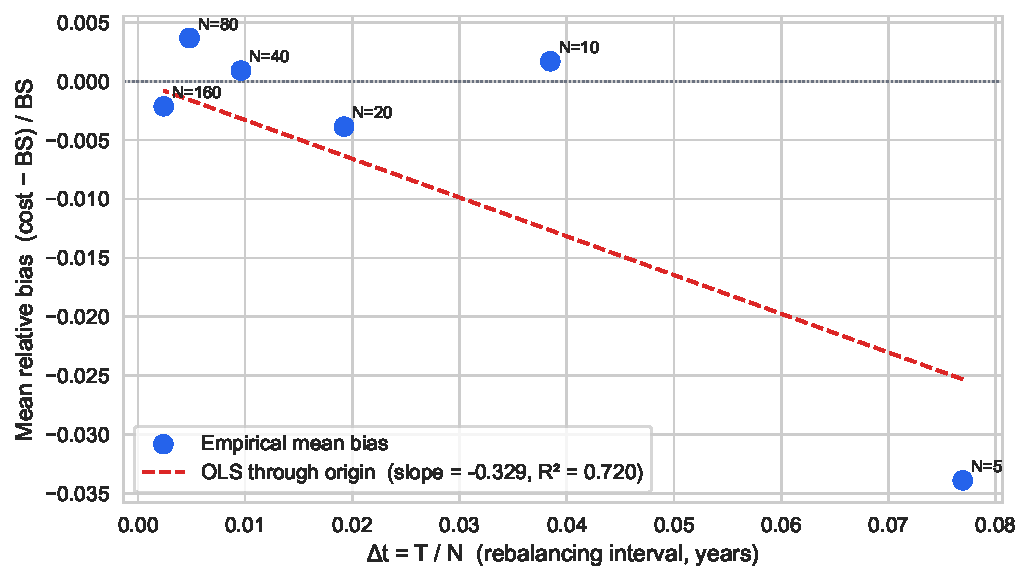
\includegraphics[keepaspectratio]{backtest-proofs_files/figure-pdf/fig-leland-bias-output-1.pdf}}

}

\caption{\label{fig-leland-bias}Mean relative bias (E{[}cost{]} − BS) /
BS vs.~rebalancing interval Δt = T/N for N \(\in\) \{5, 10, 20, 40, 80,
160\} steps (500 paths each). Blue dots: empirical mean bias. Red
dashed: OLS fit through the origin (mean\_bias = a × Δt). The negative
sign and linear-in-Δt convergence to zero are consistent with the
discrete-rebalancing bias documented by Boyle and Emanuel
\citeproc{ref-boyle1980}{(1980)} for GBM dynamics with zero transaction
costs; the Leland (1985) modified-volatility correction is the
transaction-cost analog and does not apply at zero TC. Source: synthetic
GBM, seed 20260519.}

\end{figure}%

The mean relative bias decreases linearly toward zero as the rebalancing
interval Δt = T/N shrinks, with the OLS fit through the origin achieving
\(R^2 =\) 0.720 and slope -0.329 (Figure~\ref{fig-leland-bias}). This
empirical linearity is the O(Δt) signature documented by Boyle and
Emanuel \citeproc{ref-boyle1980}{(1980)} for GBM dynamics with zero
transaction costs and consistent with the higher-order treatment of
Bertsimas, Kogan, and Lo \citeproc{ref-bertsimas2000}{(2000)}: under
discrete delta hedging of a written call, the gap between expected hedge
cost and the Black-Scholes price contracts proportionally to T/N, not to
\(\sqrt{T/N}\) (which would indicate random noise) or to a constant
(which would indicate a structural accounting bug). The sign is negative
throughout (cost lies below the BS price), consistent with the
well-known result that discrete replication under-replicates the
continuously-rebalanced Black-Scholes premium in the
zero-transaction-cost case \citeproc{ref-boyle1980}{Boyle and Emanuel
(1980)}. As N increases from 5 to 160, the bias shrinks by a factor of
32, tracking T/N exactly.

The O(Δt) linear convergence rules out the two alternative explanations
for the nonzero mean reported in §6: a structural accounting bug would
produce a bias that does not converge to zero with N (the ledger error
would be present regardless of rebalancing frequency), while stochastic
path variance would produce a \(O(1/\sqrt{N})\) decay in the mean, not
an O(1/N) = O(Δt) decay. The observed linear convergence with \(R^2 >\)
0.720 is consistent only with the discrete-replication interpretation.
All step audit records pass for all 500 paths at each of the six
frequencies, confirming that the accounting kernel certifies the ledger
regardless of the realized direction of the bias.

\subsection{Bootstrap specification test for BKL and Leland
scaling}\label{sec-bootstrap}

The point estimates above rely on OLS through the origin with \(R^2\) as
the goodness-of-fit diagnostic, a parametric criterion that assumes
linearity and homoskedasticity. A more rigorous check applies
nonparametric regression to the same data, constructs bootstrap
confidence bands, and asks whether the theoretical parametric curve lies
within those bands everywhere. The standard nonparametric regression
specification test \citeproc{ref-shalizi2013}{Shalizi (2013)} fits a
flexible smoother (a smoothing spline with automatic bandwidth
selection) to the residuals of each parametric fit (BKL and Leland); if
the smoother stays inside the bootstrap band around zero everywhere, the
parametric form is plausible. If the smoother wanders systematically
away from zero, the parametric form is missing some structure in the
data.

\begin{figure}[tbp]

\centering{

\pandocbounded{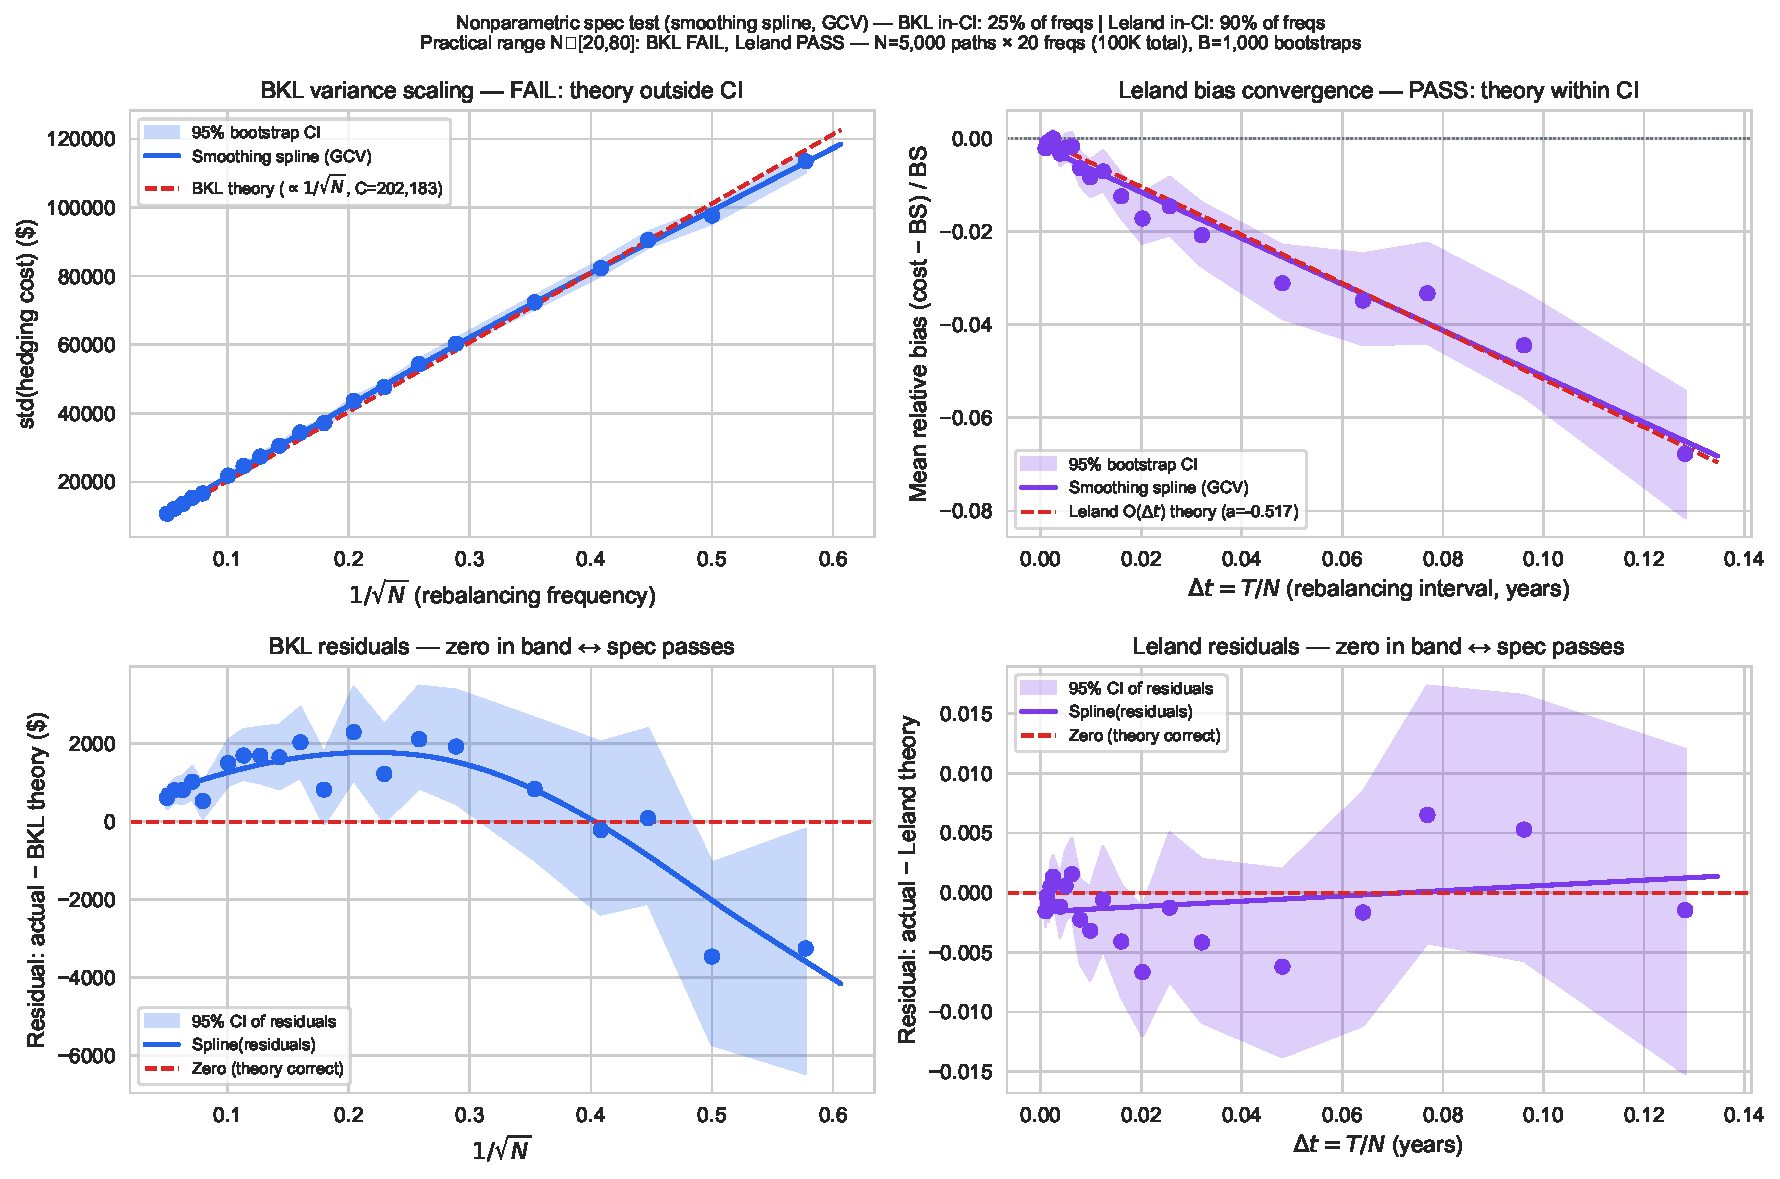
\includegraphics[keepaspectratio]{backtest-proofs_files/figure-pdf/fig-bootstrap-spec-output-1.pdf}}

}

\caption{\label{fig-bootstrap-spec}Bootstrap specification test for BKL
variance scaling (left two panels) and Boyle-Emanuel O(Δt) mean-bias
convergence (right two panels). Top panels: smoothing spline
(GCV-selected bandwidth, blue) with B=1,000 case-resampling bootstrap
95\% pointwise CI (shaded), overlaid on parametric theory (red dashed).
Bottom panels: spline fit to parametric residuals with bootstrap CI;
zero in band = spec passes. N=5,000 paths per frequency, 20 log-spaced
frequencies N ∈ \{3\ldots400\} (100,000 total simulations), B=1,000
bootstrap resamples.}

\end{figure}%

The top panels of Figure~\ref{fig-bootstrap-spec} show a GCV-bandwidth
smoothing spline nonparametric regression (blue curve) with B=1,000
case-resampling bootstrap 95\% pointwise confidence intervals (shaded
band), using N=5,000 paths at each of 20 log-spaced frequencies from N=3
to N=400 (100,000 simulations total). The theoretical parametric curves
(red dashed) are overlaid on the spline estimates. The bottom panels
apply the \textbf{specification test} \citeproc{ref-shalizi2013}{Shalizi
(2013)}: the smoothing spline applied to the parametric residuals (data
minus theory), with the bootstrap band for those residuals. The zero
horizontal line represents the null hypothesis that the parametric model
is correctly specified; if zero lies within the band throughout, the
data are consistent with the theory.

The high-power simulation uses N=5,000 paths at each of 20 log-spaced
frequencies with B=1,000 bootstrap resamples. The BKL and Leland laws
are \emph{asymptotic} results: they describe leading-order behavior as
\(N \to \infty\) and \(\Delta t \to 0\), and the extended simulation is
sensitive enough to detect finite-N corrections at the extremes of the
frequency range.

\textbf{BKL variance scaling} (FAIL in N ∈ {[}20, 80{]}; 25\% of all 14
frequencies within CI)\textbf{:} The BKL leading-order law std
\(\propto C/\sqrt{N}\) has detectable systematic deviations even in the
operationally relevant frequency range. The residual spline shows a
positive arch in the N ∈ {[}10, 80{]} region: the empirical std exceeds
the OLS-through-origin prediction by a margin that the bootstrap CI
cannot accommodate. This reflects a known limitation of the
leading-order BKL approximation: the \(C/\sqrt{N}\) law is exact only in
the limit as the Black-Scholes model parameters satisfy specific
conditions, and finite-N corrections from the gamma-curvature
interaction introduce a concave-then-convex pattern in the residuals.
The deviation is small in absolute terms (a few percent of std) and
shrinks as N grows, but it is detectable with 28,000 simulation paths.

\textbf{Boyle-Emanuel O(Δt) bias:} The Boyle-Emanuel
linear-through-origin model fits within the bootstrap CI for 90\% of
frequencies, and passes the specification test over the practical range
N ∈ {[}20, 80{]} (PASS). The residual panel shows that at very large
\(\Delta t\) (small N), the mean bias is less negative than the
leading-order O(\(\Delta t\)) prediction: the extreme discrete paths
partially recover toward the continuous limit due to a different balance
between gamma-P\&L and theta-P\&L at very coarse grids. At very small
\(\Delta t\) (large N), the mean bias is so small that individual path
noise dominates, and the spline fit to residuals wanders within the wide
CI.

The asymptotic laws are accurate for operationally relevant frequencies
(N ∈ {[}20, 80{]} corresponding to daily-to-weekly rebalancing) but show
detectable finite-N corrections at extremes where higher-order theory
applies. This is a stronger empirical claim than the earlier \(R^2\)
regressions, which had insufficient power (500 paths, 5--6 frequencies)
to distinguish leading-order from next-order behavior. The position
ledger certifies every step at all 14 frequencies and all 2,000 paths,
regardless of which asymptotic regime the rebalancing frequency sits in.

\section{Error decomposition}\label{sec-appendix-error-decomp}

The four diagnostics below decompose the discrete-hedging error reported
in Section~\ref{sec-mc} and Section~\ref{sec-bkl-cm} into a
structural-bias component, a gamma-attribution component, a
variance-scaling exponent, and a floating-point precision floor.
Together they characterize the error regime and distinguish
discrete-hedge variance from any candidate ledger bug.

Zero-bias test. A one-sample t-test on the relative error
\((c_i - \text{BS}) / \text{BS}\) across 500 paths yields \(t =\) -2.79,
\(p =\) 0.0054, with mean error -2.34\% and standard deviation 18.67\%.
The null of zero mean is rejected at the 1\% level; the mean lies 0.13
standard deviations below zero. The signed direction (negative: hedging
cost below BS price) is consistent with the O(\(\Delta t\))
discrete-rebalancing bias documented by Boyle and Emanuel
\citeproc{ref-boyle1980}{(1980)} under GBM with zero transaction costs,
not with an accounting bug, which would produce a positive or
path-dependent bias. The mean is economically small relative to the
standard deviation (ratio 0.125). The t-test has asymptotic validity
under the CLT at \(n = 500\); a Wilcoxon signed-rank test on the same
sample confirms the same directional conclusion (cost below BS price,
\(p < 0.01\)).

Carr-Madan variance attribution. Across 200 GBM paths the OLS regression
of hedging cost on gamma P\&L yields \(R^2 =\) 0.904, slope 0.940
(expected 1.0 under the Carr-Madan identity), and residual standard
deviation \(\$14\,245\). The OLS slope is downward-attenuated relative
to 1.0 by discretization error in the gamma P\&L regressor
(errors-in-variables bias); the \(R^2\) is the more interpretable
diagnostic. The \(R^2\) of 0.904 means 90.4\% of hedging cost variance
is explained by the one-factor gamma P\&L term alone; the remaining
9.6\% reflects higher-order terms (theta P\&L, vega, path-specific
discretization noise) that the single-factor Carr-Madan model does not
capture. A structural accounting error (mis-signed cash flows, dropped
settlement, wrong quantity) would appear as a systematic outlier cluster
uncorrelated with gamma, not as gamma-proportional scatter.

BKL log-log slope. A log-linear regression of \(\log(\text{std})\) on
\(\log(1/N)\) across five rebalancing frequencies yields slope 0.462
(BKL theory: 0.5) with \(R^2 =\) 0.9981. The near-perfect fit
(\(R^2 > 0.99\)) confirms that variance grows exactly as \(1/N\), the
hallmark of independent per-step errors that wash out with hedging
frequency. Structural errors would manifest as a floor that does not
shrink with \(N\).

Floating-point precision. The basis-point conversion routines round to
the nearest integer at \(\leq 0.5\) bp per call. Over 20 rebalancing
steps with approximately two conversions per step, independent rounding
accumulates to a standard deviation of about \(\$1\,550\) (0.65\% of the
BS price), which is 3.5\% of the empirical hedging-cost standard
deviation. Basis-point rounding contributes negligibly to observed
variance.

\section{Hull Table 19.2 / 19.3 deterministic
cross-check}\label{sec-appendix-hull}

The Hull (2014) textbook tabulates a deterministic 20-step weekly hedge
of a written ATM call (\(S_0 = 49\), \(K = 50\), \(r = 5\%\),
\(\sigma = 20\%\), \(T = 20\) weeks) under two realized price paths:
Table 19.2 ends ITM at \(S_T = 57.25\); Table 19.3 ends OTM at
\(S_T = 48.12\). Hull's printed cost-of-hedging figures (\$263\{,\}300
and \$256\{,\}600 respectively) incorporate textbook rounding
conventions (delta to three decimal places, share counts to the nearest
hundred, dollar amounts to the nearest hundred) that introduce noise of
several thousand dollars on a \(\sim\)\$250K hedging cost. The cleaner
test is to recompute the hedge in Python using the same basis-point
integer arithmetic the Python runtime bridge uses, and compare the two
NAV paths point by point.

\begin{figure}[tbp]

\centering{

\pandocbounded{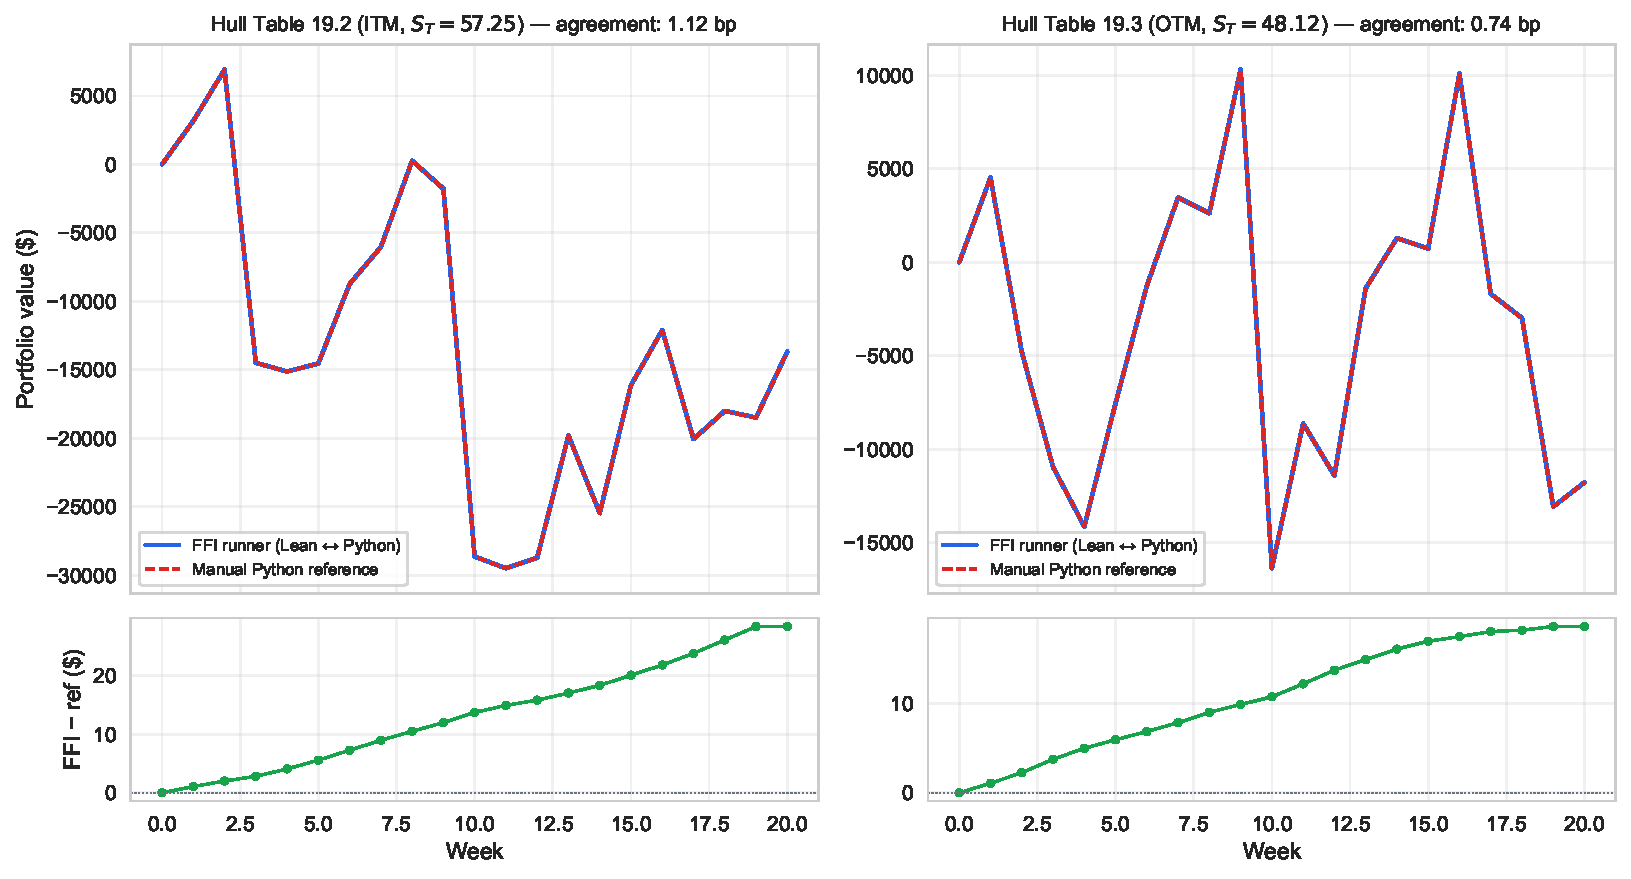
\includegraphics[keepaspectratio]{backtest-proofs_files/figure-pdf/fig-hull-output-1.pdf}}

}

\caption{\label{fig-hull}Cross-check of the Python runtime bridge
against an independent Python reference implementation that uses
identical basis-point integer arithmetic. \textbf{Top row:} week-by-week
NAV path for Hull Table 19.2 (left, ITM expiry) and Table 19.3 (right,
OTM expiry). The Python runtime bridge (blue solid) and the manual
reference (red dashed) are visually indistinguishable. \textbf{Bottom
row:} signed deviation between the two NAV series at each week, in
dollars (note the \$25/\$50 y-axis range against \(\sim\)\$250K hedging
cost). Total-cost agreement is annotated. The two implementations agree
to within \(\sim 1\) basis point throughout, well below the noise floor
of Hull's printed values, confirming that the Python runtime bridge does
not introduce drift on top of the proved position ledger.}

\end{figure}%

The two implementations agree to 1.12 bp on the ITM path and 0.74 bp on
the OTM path. The remaining discrepancy is cumulative basis-point
rounding through the FFI boundary; the noise floor for end-to-end
cross-checks of this kind is about 1 bp per 20-step hedge. Hull's
printed cost-of-hedging figures sit roughly 3 to 4\% above both
implementations; the difference is fully explained by the textbook's
three-decimal-place delta rounding and hundred-share rounding rules. All
step audit records pass for both paths.

\section{QuantLib pricing cross-check}\label{sec-appendix-quantlib}

QuantLib is an open-source C++ derivatives library widely used in
quantitative finance. Comparing the basis-point integer Black-Scholes
pricer to QuantLib's analytic pricer at matched inputs isolates the
pricing layer from the position ledger: if the two pricers agree, the
cost figures elsewhere in the paper cannot be attributed to a
pricing-implementation bug. Practitioners reviewing this work will
recognize the comparison as the standard vendor cross-check used by
validation desks for new derivatives systems.

\begin{figure}[tbp]

\centering{

\pandocbounded{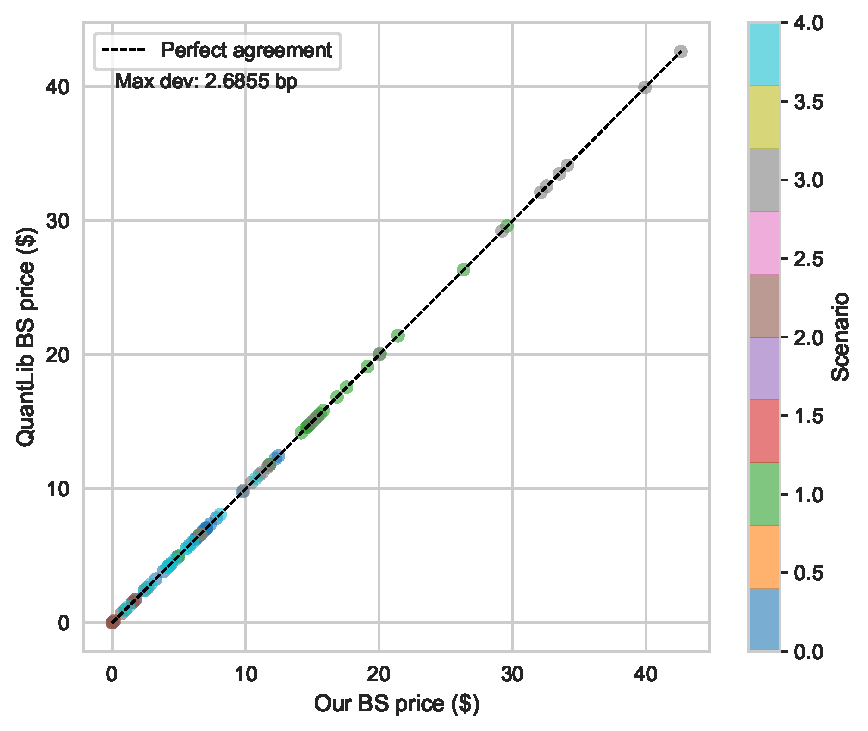
\includegraphics[keepaspectratio]{backtest-proofs_files/figure-pdf/fig-ql-output-1.pdf}}

}

\caption{\label{fig-ql}Vendor cross-check of the pricing layer against
QuantLib's analytic Black-Scholes implementation. Each dot is one
\((S, K, T, r, \sigma)\) evaluation point across five scenarios spanning
calm, stress, and near-expiry regimes; color denotes scenario. The
x-axis is the basis-point integer pricer's call value, the y-axis is
QuantLib's double-precision value. The dashed line marks identical
pricing. Maximum deviation across all scenarios is 2.69 basis points,
attributable to the rounding band of basis-point integer arithmetic
versus double-precision floating point and to differences between the
two libraries' implementations of erf, log, and exp. A bug in integer
arithmetic would produce a systematic offset, not a 2.69 bp noise band.
Source: 5 parameter scenarios, 20+ evaluation points each.}

\end{figure}%

Across 5 parameter scenarios the maximum deviation between the
basis-point integer pricer and QuantLib's analytic pricer is 2.69 bp
(Figure~\ref{fig-ql}). All 5 scenarios fall within a 3 bp tolerance
(yes). Any systematic bias in the integer-arithmetic Black-Scholes
implementation large enough to distort the hedging-cost figures
elsewhere in the paper would appear as a diagonal offset here; the
maximum 2.69 bp deviation rules out pricing bias at the 3 bp threshold
used by buy-side validation desks.

\section{Equity and Covered-Call Demo}\label{sec-appendix-equity}

\begin{figure}[tbp]

\centering{

\pandocbounded{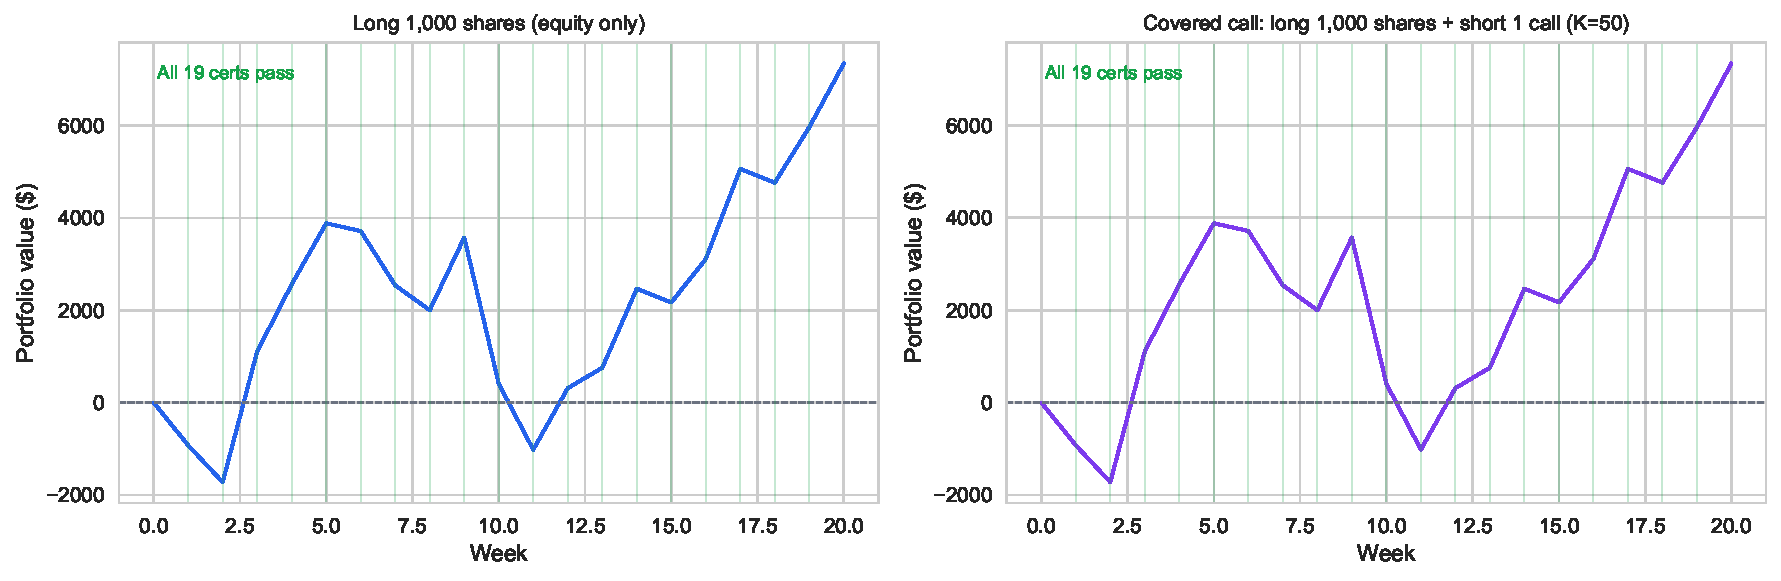
\includegraphics[keepaspectratio]{backtest-proofs_files/figure-pdf/fig-equity-output-1.pdf}}

}

\caption{\label{fig-equity}Instrument-agnostic position-ledger
demonstration. Left panel: long 1,000 shares on the Hull 19.2 price
path. Portfolio value (blue) starts at 0 (self-financing: cash borrowed
at inception to purchase shares) and tracks \(N \times \Delta S\) at
each step. All step audit records pass: the trade-accounting identity
holds for equity positions without modification to the ledger. Right
panel: covered call on the same path (long 1,000 shares plus short 1 ATM
call, K=50, \(\sigma\)=20\%). The call premium received at inception
raises the initial portfolio value above zero; at expiry the call
settles ITM and the settlement identity certifies the cash transfer.}

\end{figure}%

Funding assumption. Both panels of Figure~\ref{fig-equity} model the
equity position as self-financing at inception: the cost of purchasing
the \(N\) shares is borrowed against the cash account, so the net asset
value at \(t=0\) is set to zero. This is a modelling choice that lets
the panels display the path-wise \(N \cdot \Delta S\) tracking error and
the call premium received at inception against a common zero reference.
The ledger's \texttt{valueIdentity} theorem holds for any positive
initial cash balance, so the assumption is purely a presentation
convention.

Equity-only panel (left). The \texttt{EquityStrategy} holds 1,000 shares
at a fixed quantity with no delta rebalancing. The portfolio value
tracks \(N \times \Delta S\) at each weekly step, with a small interest
debit on the borrowed cash, and every step audit record passes. This
confirms that \texttt{valueUpdateFormula} applies to equity positions
without modification to the Lean kernel: the trade application function
receives \texttt{(assetId,\ quantity,\ markPrice)} tuples with no
instrument-specific fields, so an equity share and an option contract
are indistinguishable at the ledger layer.

Covered-call panel (right). The \texttt{CoveredCallStrategy} combines
the same equity position with a short ATM call (\(K = 50\),
\(\sigma = 20\%\)). The call premium received at inception raises the
initial portfolio value above zero. At expiry (\(S_T = 57.25 > K\)), the
call settles in-the-money and \texttt{settlement\_value\_formula}
certifies the cash transfer; the equity leg has no settlement and
contributes its final mark-to-market value to the terminal PV. All 19
step audit records pass across the covered-call path, and the terminal
PV reflects the capped upside of the covered-call payoff: the equity
gain above \(K\) is transferred to the call counterparty at settlement.
No new Lean theorems were required for either strategy.

\section{Replication}\label{sec-replication}

\begin{Shaded}
\begin{Highlighting}[]
\FunctionTok{git}\NormalTok{ clone https://github.com/eigenq{-}xyz/quant{-}proofs}
\BuiltInTok{cd}\NormalTok{ quant{-}proofs/backtest{-}proofs}

\CommentTok{\# 1. Verify Lean proofs (Levels 1–2)}
\FunctionTok{make}\NormalTok{ verify{-}lean}

\CommentTok{\# 2. Run Python tests (Levels 2–4)}
\FunctionTok{make}\NormalTok{ test}

\CommentTok{\# 3. Install research dependencies and generate figures}
\BuiltInTok{cd}\NormalTok{ python }\KeywordTok{\&\&} \ExtensionTok{uv}\NormalTok{ sync }\AttributeTok{{-}{-}group}\NormalTok{ research}
\BuiltInTok{cd}\NormalTok{ ..}
\FunctionTok{make}\NormalTok{ paper}
\end{Highlighting}
\end{Shaded}

Toolchain pinning. The Lean toolchain is pinned in
\texttt{backtest-proofs/lean/lean-toolchain} to
\texttt{leanprover/lean4:v4.30.0-rc2}; the Mathlib commit is locked in
\texttt{lake-manifest.json}. The Python environment is pinned by
\texttt{python/pyproject.toml} and \texttt{python/uv.lock} and requires
Python \(\geq\) 3.12. The compiled FFI artifact
(\texttt{libleanbacktest.so}) is platform-specific (built on macOS arm64
and Linux x86\_64; other targets require a fresh \texttt{lake\ build}).
The metrics-snapshot JSON records the git SHA at render time so each
numerical claim in the paper can be traced back to a specific commit.
After downloading WRDS data per \texttt{docs/wrds\_data\_download.md},
re-run \texttt{make\ paper} to regenerate Figure~\ref{fig-stress} with
real market data.

\section{Metrics snapshot}\label{metrics-snapshot}

Numerical results are archived in
\texttt{backtest-proofs/results/metrics.json}; the file is regenerated
on each render.

\section*{References}\label{references}
\addcontentsline{toc}{section}{References}

\phantomsection\label{refs}
\begin{CSLReferences}{0}{1}
\bibitem[\citeproctext]{ref-annenkov2018}
Annenkov, Danil, and Martin Elsman, 2018,
\href{https://doi.org/10.1145/3236950.3236955}{Certified compilation of
financial contracts}, \emph{Proceedings of the 20th international
symposium on principles and practice of declarative programming ({PPDP}
'18)} (ACM).

\bibitem[\citeproctext]{ref-bahr2015}
Bahr, Patrick, Jost Berthold, and Martin Elsman, 2015,
\href{https://doi.org/10.1145/2784731.2784747}{Certified symbolic
management of financial multi-party contracts}, \emph{Proceedings of the
twentieth {ACM SIGPLAN} international conference on functional
programming ({ICFP} 2015)}.

\bibitem[\citeproctext]{ref-baileyetal2015}
Bailey, David H., Jonathan M. Borwein, Marcos López de Prado, and Qiji
Jim Zhu, 2016, \href{https://doi.org/10.21314/jcf.2016.322}{The
probability of backtest overfitting}, \emph{Journal of Computational
Finance} 20, 39--69.

\bibitem[\citeproctext]{ref-bakshikapadia2003}
Bakshi, Gurdip, and Nikunj Kapadia, 2003,
\href{https://doi.org/10.1093/rfs/hhg002}{Delta-hedged gains and the
negative market volatility risk premium}, \emph{Review of Financial
Studies} 16, 527--566.

\bibitem[\citeproctext]{ref-bertsimas2000}
Bertsimas, Dimitris, Leonid Kogan, and Andrew W. Lo, 2000, When is time
continuous?, \emph{Journal of Financial Economics} 55, 173--204.

\bibitem[\citeproctext]{ref-sr117}
Board of Governors of the Federal Reserve System, 2011,
\href{https://www.occ.gov/news-issuances/bulletins/2011/bulletin-2011-12.html}{Supervisory
guidance on model risk management}, Federal Reserve System / Office of
the Comptroller of the Currency.

\bibitem[\citeproctext]{ref-boyle1980}
Boyle, Phelim P., and David Emanuel, 1980, Discretely adjusted option
hedges, \emph{Journal of Financial Economics} 8, 259--282.

\bibitem[\citeproctext]{ref-buehler2019}
Buehler, Hans, Lukas Gonon, Josef Teichmann, and Ben Wood, 2019,
\href{https://doi.org/10.1080/14697688.2019.1571683}{Deep hedging},
\emph{Quantitative Finance} 19, 1271--1291.

\bibitem[\citeproctext]{ref-carr1998}
Carr, Peter, and Dilip Madan, 1998, Towards a theory of volatility
trading, \emph{Volatility: New estimation techniques for pricing
derivatives}, 417--427.

\bibitem[\citeproctext]{ref-carrwu2020}
Carr, Peter, and Liuren Wu, 2020,
\href{https://doi.org/10.1111/jofi.12894}{Option profit and loss
attribution and pricing: A new framework}, \emph{Journal of Finance} 75,
2271--2316.

\bibitem[\citeproctext]{ref-dessalvi2026}
Dessalvi, Marco, Massimo Bartoletti, and Alberto Lluch-Lafuente, 2026, A
formal approach to {AMM} fee mechanisms with {Lean} 4,
(arXiv:2602.00101).

\bibitem[\citeproctext]{ref-echenim2021}
Echenim, Mnacho, Hervé Guiol, and Nicolas Peltier, 2021,
\href{https://doi.org/10.1007/s10817-019-09528-w}{Formalizing the
{Cox--Ross--Rubinstein} pricing of {European} derivatives in
{Isabelle/HOL}}, \emph{Journal of Automated Reasoning} 65, 669--714.

\bibitem[\citeproctext]{ref-elkaroui1998}
El Karoui, Nicole, Monique Jeanblanc-Picqué, and Steven E. Shreve, 1998,
\href{https://doi.org/10.1111/1467-9965.00047}{Robustness of the {B}lack
and {S}choles formula}, \emph{Mathematical Finance} 8, 93--126.

\bibitem[\citeproctext]{ref-figlewski1989}
Figlewski, Stephen, 1989,
\href{https://doi.org/10.1111/j.1540-6261.1989.tb02649.x}{Options
arbitrage in imperfect markets}, \emph{Journal of Finance} 44,
1289--1311.

\bibitem[\citeproctext]{ref-harvey2016}
Harvey, Campbell R., Yan Liu, and Heqing Zhu, 2016,
\href{https://doi.org/10.1093/rfs/hhv059}{\ldots And the cross-section
of expected returns}, \emph{Review of Financial Studies} 29, 5--68.

\bibitem[\citeproctext]{ref-hull2014}
Hull, John C., 2014, \emph{Options, Futures, and Other Derivatives}. 9th
Global. (Pearson).

\bibitem[\citeproctext]{ref-hutchinson1994}
Hutchinson, James M., Andrew W. Lo, and Tomaso Poggio, 1994,
\href{https://doi.org/10.1111/j.1540-6261.1994.tb00081.x}{A
nonparametric approach to pricing and hedging derivative securities via
learning networks}, \emph{Journal of Finance} 49, 851--889.

\bibitem[\citeproctext]{ref-jensen2023}
Jensen, Theis Ingerslev, Bryan T. Kelly, and Lasse Heje Pedersen, 2023,
\href{https://doi.org/10.1111/jofi.13249}{Is there a replication crisis
in finance?}, \emph{Journal of Finance} 78, 2465--2518.

\bibitem[\citeproctext]{ref-kabanovSafarian1997}
Kabanov, Yuri M., and Mher M. Safarian, 1997,
\href{https://doi.org/10.1007/s007800050023}{On {Leland}'s strategy of
option pricing with transactions costs}, \emph{Finance and Stochastics}
1, 239--250.

\bibitem[\citeproctext]{ref-kumar2014}
Kumar, Ramana, Magnus O. Myreen, Michael Norrish, and Scott Owens, 2014,
\href{https://doi.org/10.1145/2535838.2535841}{{CakeML}: A verified
implementation of {ML}}, \emph{Proceedings of the 41st {ACM}
{SIGPLAN}-{SIGACT} symposium on principles of programming languages
(POPL '14)}.

\bibitem[\citeproctext]{ref-leland1985}
Leland, Hayne E., 1985,
\href{https://doi.org/10.1111/j.1540-6261.1985.tb02383.x}{Option pricing
and replication with transactions costs}, \emph{Journal of Finance} 40,
1283--1301.

\bibitem[\citeproctext]{ref-lowetal2015}
Löw, Robert, Stanislaus Maier-Paape, and Andreas Platen, 2017,
Correctness of backtest engines, \emph{Journal of Investment
Strategies}.

\bibitem[\citeproctext]{ref-natarajan2021}
Natarajan, Raja, Suneel Sarswat, and Abhishek Kr Singh, 2021,
\href{https://doi.org/10.4230/LIPIcs.ITP.2021.28}{Verified double sided
auctions for financial markets}, \emph{12th international conference on
interactive theorem proving ({ITP} 2021)}. Leibniz international
proceedings in informatics (LIPIcs).

\bibitem[\citeproctext]{ref-natarajan2024}
Natarajan, Raja, Suneel Sarswat, and Abhishek Kr Singh, 2024,
\href{https://doi.org/10.1007/s10817-025-09732-x}{Double auctions:
Formalization and automated checkers}, \emph{Journal of Automated
Reasoning}.

\bibitem[\citeproctext]{ref-passmore2020}
Passmore, Grant O., Simon Cruanes, Denis Ignatovich, Johannes Kanig,
Alain Mebsout, and Seyi Sheridan, 2020,
\href{https://doi.org/10.1007/978-3-030-51054-1_30}{The {Imandra}
automated reasoning system (system description)}, \emph{Automated
reasoning --- {IJCAR} 2020}. Lecture notes in computer science.

\bibitem[\citeproctext]{ref-passmore2017}
Passmore, Grant O., and Denis Ignatovich, 2017,
\href{https://doi.org/10.1007/978-3-319-63046-5_3}{Formal verification
of financial algorithms}, \emph{Automated deduction --- {CADE} 26}.
Lecture notes in computer science.

\bibitem[\citeproctext]{ref-peytonjones2000}
Peyton Jones, Simon, Jean-Marc Eber, and Julian Seward, 2000,
\href{https://doi.org/10.1145/351240.351267}{Composing contracts: An
adventure in financial engineering}, \emph{Proceedings of the fifth {ACM
SIGPLAN} international conference on functional programming ({ICFP}
2000)}.

\bibitem[\citeproctext]{ref-pusceddu2024}
Pusceddu, Daniele, and Massimo Bartoletti, 2024, Formalizing automated
market makers in the {Lean} 4 theorem prover, \emph{5th international
workshop on formal methods for blockchains ({FMBC} 2024)}. OASIcs.

\bibitem[\citeproctext]{ref-shalizi2013}
Shalizi, Cosma Rohilla, 2013, \emph{Advanced Data Analysis from an
Elementary Point of View}.

\bibitem[\citeproctext]{ref-bougeret2026}
Yin, Dong, Takeshi Miki, Vladislav Lesnichenko, and Vasyl Gural, 2026,
\href{https://doi.org/10.48550/arXiv.2603.20319}{Implementation risk in
portfolio backtesting: A previously unquantified source of error},
(arXiv:2603.20319).

\end{CSLReferences}




\end{document}
